\documentclass[dvipdfmx, unicode]{beamer}

\usepackage{../style/beamerthememetropolis}

% 数式使えるよん
\usepackage{amsmath}
\usepackage{amssymb}
\usepackage{amsfonts}
\usepackage{mathtools}
\usepackage{amsthm}
\usepackage{yhmath}
\mathtoolsset{showonlyrefs=True}
\usepackage{cancel}

% グラフや図形
\usepackage{tikz}
\usetikzlibrary{intersections,calc,arrows.meta,angles}

% 画像挿入用
\usepackage{graphicx}
\usepackage{float}
\usepackage{caption} % 図を横に並べる
\usepackage[subrefformat=parens]{subcaption}
\captionsetup{compatibility=false}
\usepackage[export]{adjustbox}

% 表関連
\usepackage{diagbox}
\usepackage{pict2e}
\usepackage{multirow} % 表の縦に結合

% ソースコード用
\usepackage{listings}
\renewcommand{\lstlistingname}{}

\definecolor{OliveGreen}{rgb}{0.0,0.6,0.0}
\definecolor{Orange}{rgb}{0.89,0.55,0}
\definecolor{SkyBlue}{rgb}{0.28, 0.28, 0.95}

\lstset{
  basicstyle={\ttfamily\tiny}, % 使用フォント
  classoffset=1,
  identifierstyle={},
  commentstyle={},
  keywordstyle={\bfseries},
  ndkeywordstyle={},
  stringstyle={\ttfamily},
  frame={trBl},
  framesep={2pt},
  breaklines=true,
  columns=[l]{fullflexible},
  numbers=left,
  numberstyle={\tiny},
  stepnumber=1,
  tabsize=2,
  keywordstyle={\color{blue}}, %キーワード(int, ifなど)の書体指定
  commentstyle={\color{OliveGreen}}, %注釈の書体
  stringstyle={\color{Orange}}, %文字列
  showstringspaces=false,  %文字列中の半角スペースを表示させない
  keepspaces=true,
}

\usepackage{bxdpx-beamer}

\title{
  \bfseries Improving The Usability of KeTCindy\\
  and Its Effective Use in Education.
}
\subtitle{
  KeTCindyの利便性向上と効果的な教育利用に向けて
}
\author{
  Masaki Suzuki, So Ogino, Ryota Ono\\
  Kenshin Katayama, Kosuke Fujita
}
\date{\today}
\institute[]{National Institute of Technology, Numazu College\\Control and Computer Engineering}

\begin{document}

\frame{\maketitle}

\begin{frame}[t]{\bfseries Outline}
  \tableofcontents
\end{frame}

\section{KeTCindy Web Document}

\begin{frame}[t]{\bfseries KeTCindy Web Document}
  Problems in spreading KeTCindy:
  \begin{itemize}
    % \pause
    \item Difficult to install KeTCindy.
    \item There is little information about KeTCindy on the web.\\
          % \pause
          $\rightarrow$ Searching the web will not get any results.
    \item Difficult to search about functions or sample codes
          because the reference is in PDF format.
  \end{itemize}
  It has three main elements:
  \begin{itemize}
    % \pause
    \item KeTCindy Auto Installer
          % \pause
    \item KeTCindy Web Reference
          % \pause
    \item KeTCindyChat
  \end{itemize}
\end{frame}

\subsection{KeTCindy Auto Installer}

\begin{frame}[t]{\bfseries KeTCindy Auto Installer}
  % Just press the install button to start using.
  \begin{columns}[T]
    % \begin{column}{0.7\linewidth}
    %   \begin{itemize}
    %     % \pause
    %     \item Created using C\#(.NET Framework).
    %           % \pause
    %     \item Just a repeated download of the necessary software and execution of that file.
    %           % \pause
    %     \item Just press the install buton to start using.
    %           % \pause
    %           % \item Sometimes it doesn't work because of antivirus software, so it was currently being fixing as needed.
    %   \end{itemize}
    % \end{column}
    \begin{column}{0.4\linewidth}
      
\includegraphics[width=1.0\linewidth]{img/AutoInstaller/C_Sharp_Icon.png}
    \end{column}
    \begin{column}{0.4\linewidth}
      
\includegraphics[width=1.0\linewidth]{img/AutoInstaller/Microsoft_.NET_logo.png}
    \end{column}
    % \begin{column}{0.3\linewidth}
    %   % 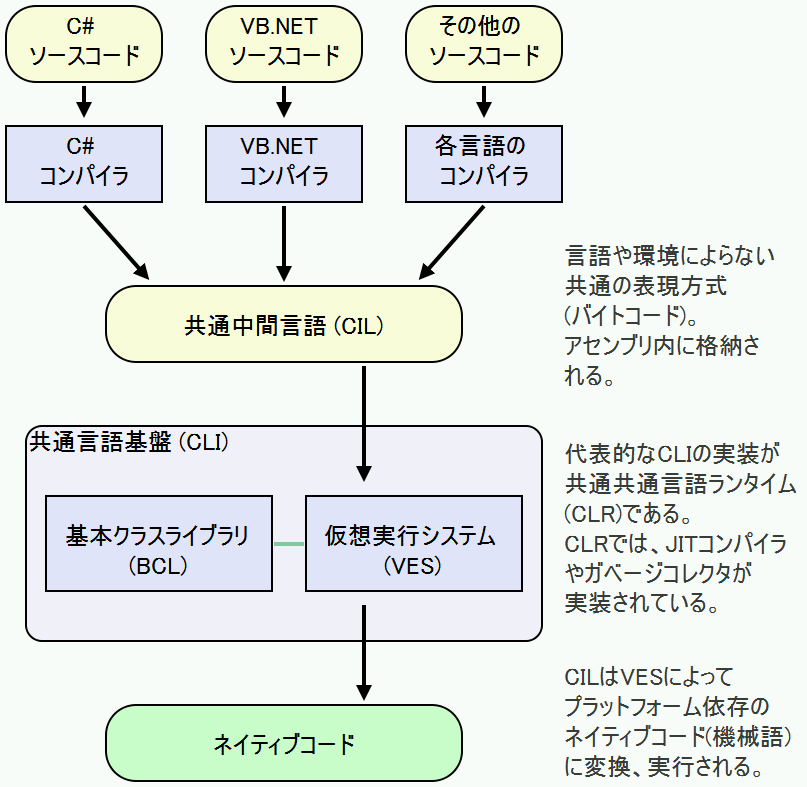
\includegraphics[width=1.0\linewidth]{img/AutoInstaller/Diagram_of_Common_Language_Infrastructure.png}

    % \end{column}
  \end{columns}
  
\includegraphics[width=1.0\linewidth]{img/AutoInstaller/Windows_logo.png}
\end{frame}

\begin{frame}{\bfseries KeTCindy Auto Installer}
  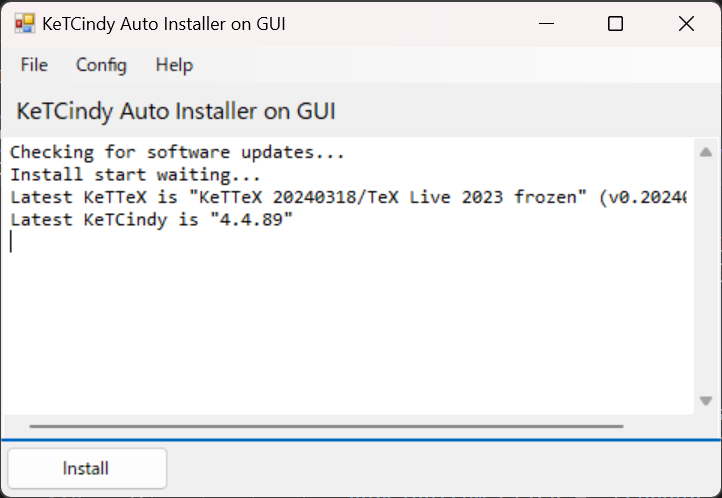
\includegraphics[width=1.0\linewidth]{img/AutoInstaller/installer_2.png}
\end{frame}

\begin{frame}{\bfseries KeTCindy Auto Installer}
  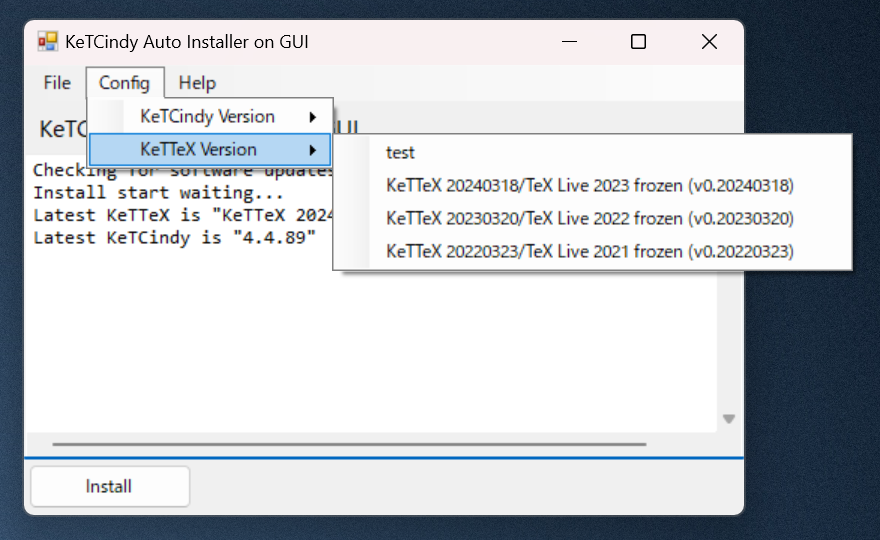
\includegraphics[width=1.0\linewidth]{img/AutoInstaller/installer_1.png}
\end{frame}

\subsection{KeTCindy Web Reference}

\begin{frame}[t]{\bfseries KeTCindy Web Reference}
  \begin{itemize}
    \item Made using Docusaurus.
    \item This reference allows users move the graphs.
    \item A comfortable search system using Algolia.
  \end{itemize}
  % 
\includegraphics[width=\linewidth]{img/Reference/Algolia_logo_full_blue.png}
\end{frame}

\begin{frame}[fragile]{\bfseries KeTCindy Web Reference}
  Powered by MDX.
  \begin{lstlisting}
## `Beziersmooth(name, node_list, [option] )`
節点間を3次ベジェ曲線でスムーズに結んだ曲線を描く.
#### 説明
節点をはさむ制御点は1直線上にとる(したがって, 1つは半自由点で, 直線上しか動けない).
制御点は自動的に配置される. その後, 節点や制御点を動かして, 描きたいものにする。  

import Beziersmooth_draw from "!!raw-loader!./code/Beziersmooth/Draw.txt"
import Beziersmooth_init from "!!raw-loader!./code/Beziersmooth/Init.txt"
import Beziersmooth_KeyTyped from "!!raw-loader!./code/Beziersmooth/KeyTyped.txt"

<CodeBox 
    Title="Beziersmooth"
    Draw={Beziersmooth_draw}
    Initialization={Beziersmooth_init}
    KeyTyped={Beziersmooth_KeyTyped}
    Frame={"/ResultImg/03_01_02_03/Beziersmoothjson.html"}
/>
  \end{lstlisting}
\end{frame}

\begin{frame}[t]{\bfseries KeTCindy Web Reference}
  \url{https://ketcindy-web-docs.vercel.app/}
  % \begin{columns}[T]
  %   \begin{column}{0.5\linewidth}
  %   \end{column}
  %   \begin{column}{0.5\linewidth}
  %     
\includegraphics[width=\linewidth]{img/Reference/Referece_QR.png}
  %   \end{column}
  % \end{columns}
  \centering
  
\includegraphics[scale=0.75]{img/Reference/Referece_QR.png}
\end{frame}

\subsection{KeTCindy Chat}

\begin{frame}[t]{\bfseries KeTCindyChat}
  \begin{itemize}
    \item Generate KeTChindy code interectively.
    \item Send questions or requests via chat.
  \end{itemize}
  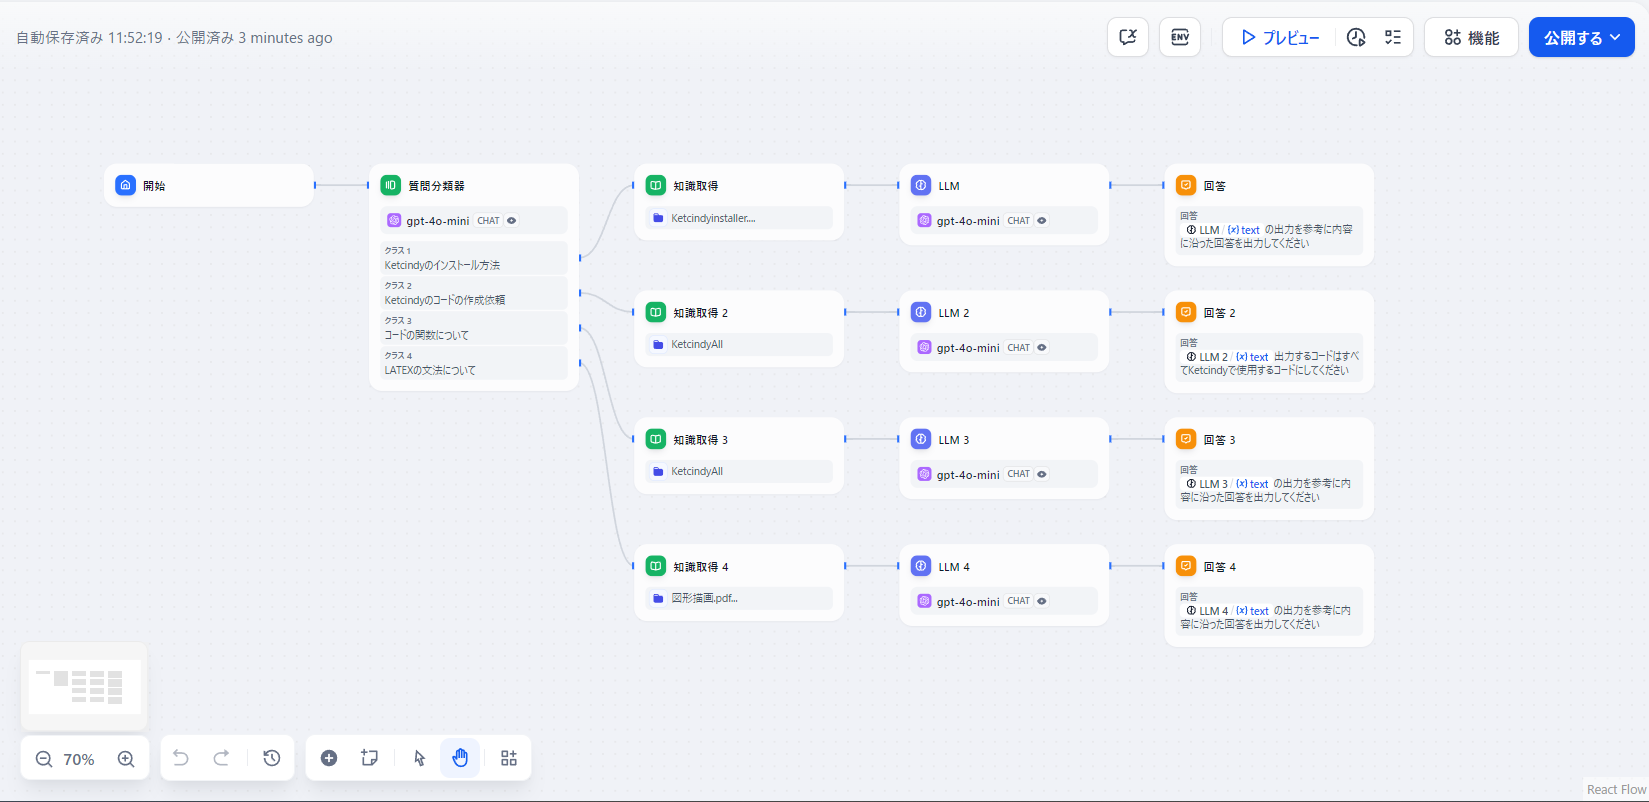
\includegraphics[width=\linewidth]{img/KeTCindyChat/appabout.png}
  % 私たちはKeTCindyのコードを対話形式で生成できる「KeTCindyChat」を開発した.
  % これにより, ユーザーはチャット形式で質問やリクエストを入力し,
  % リアルタイムでKeTCindyのコードを生成することができるようになるだろう。
  % \begin{columns}[T]
  %   \begin{column}{0.5\linewidth}
  %     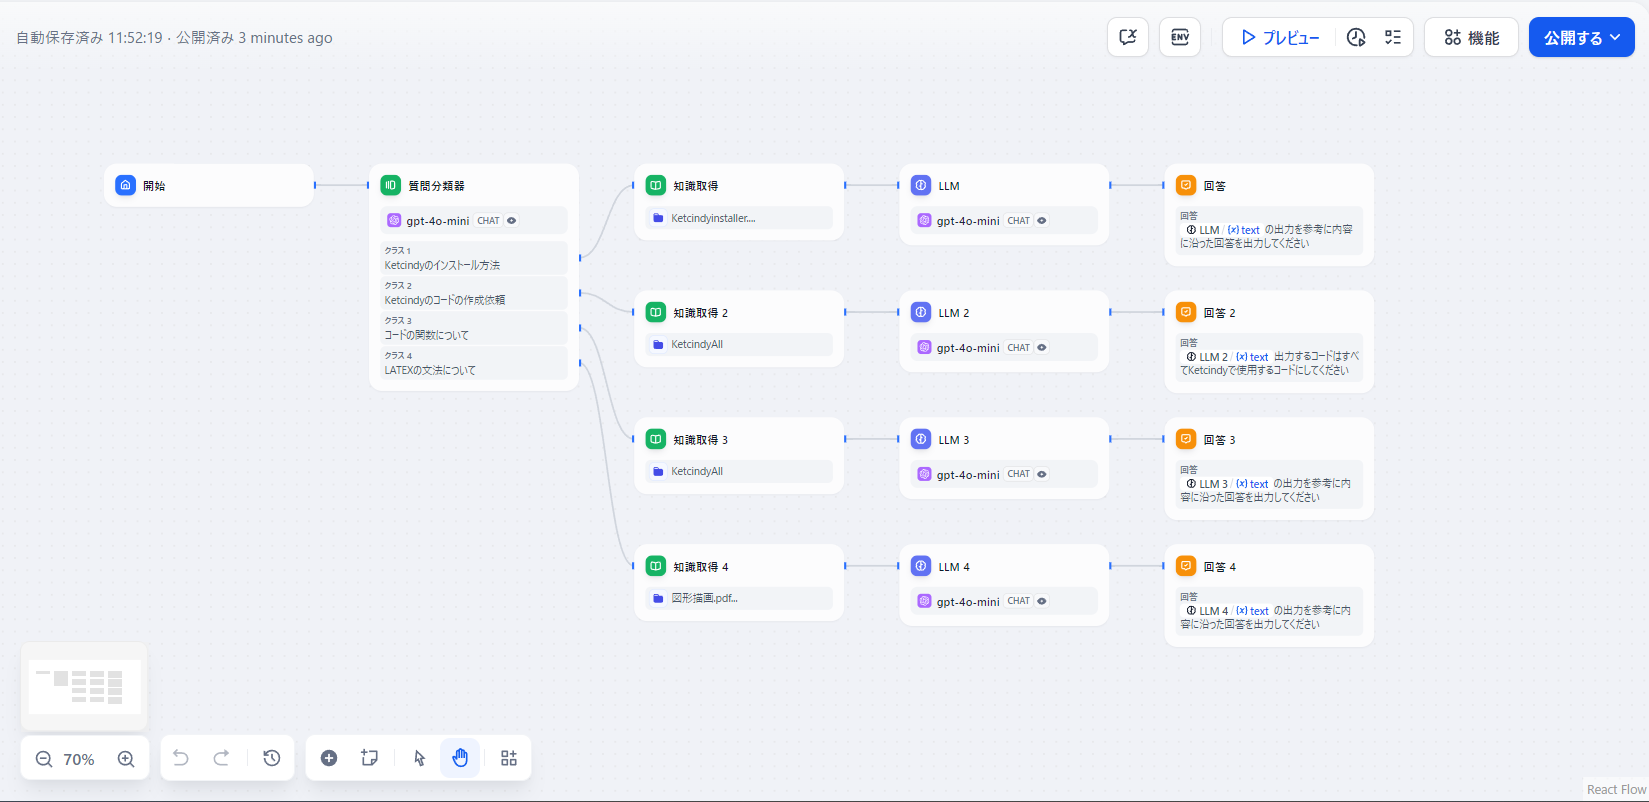
\includegraphics[width=\linewidth]{img/KeTCindyChat/appabout.png}
  %   \end{column}
  %   \begin{column}{0.5\linewidth}
  %     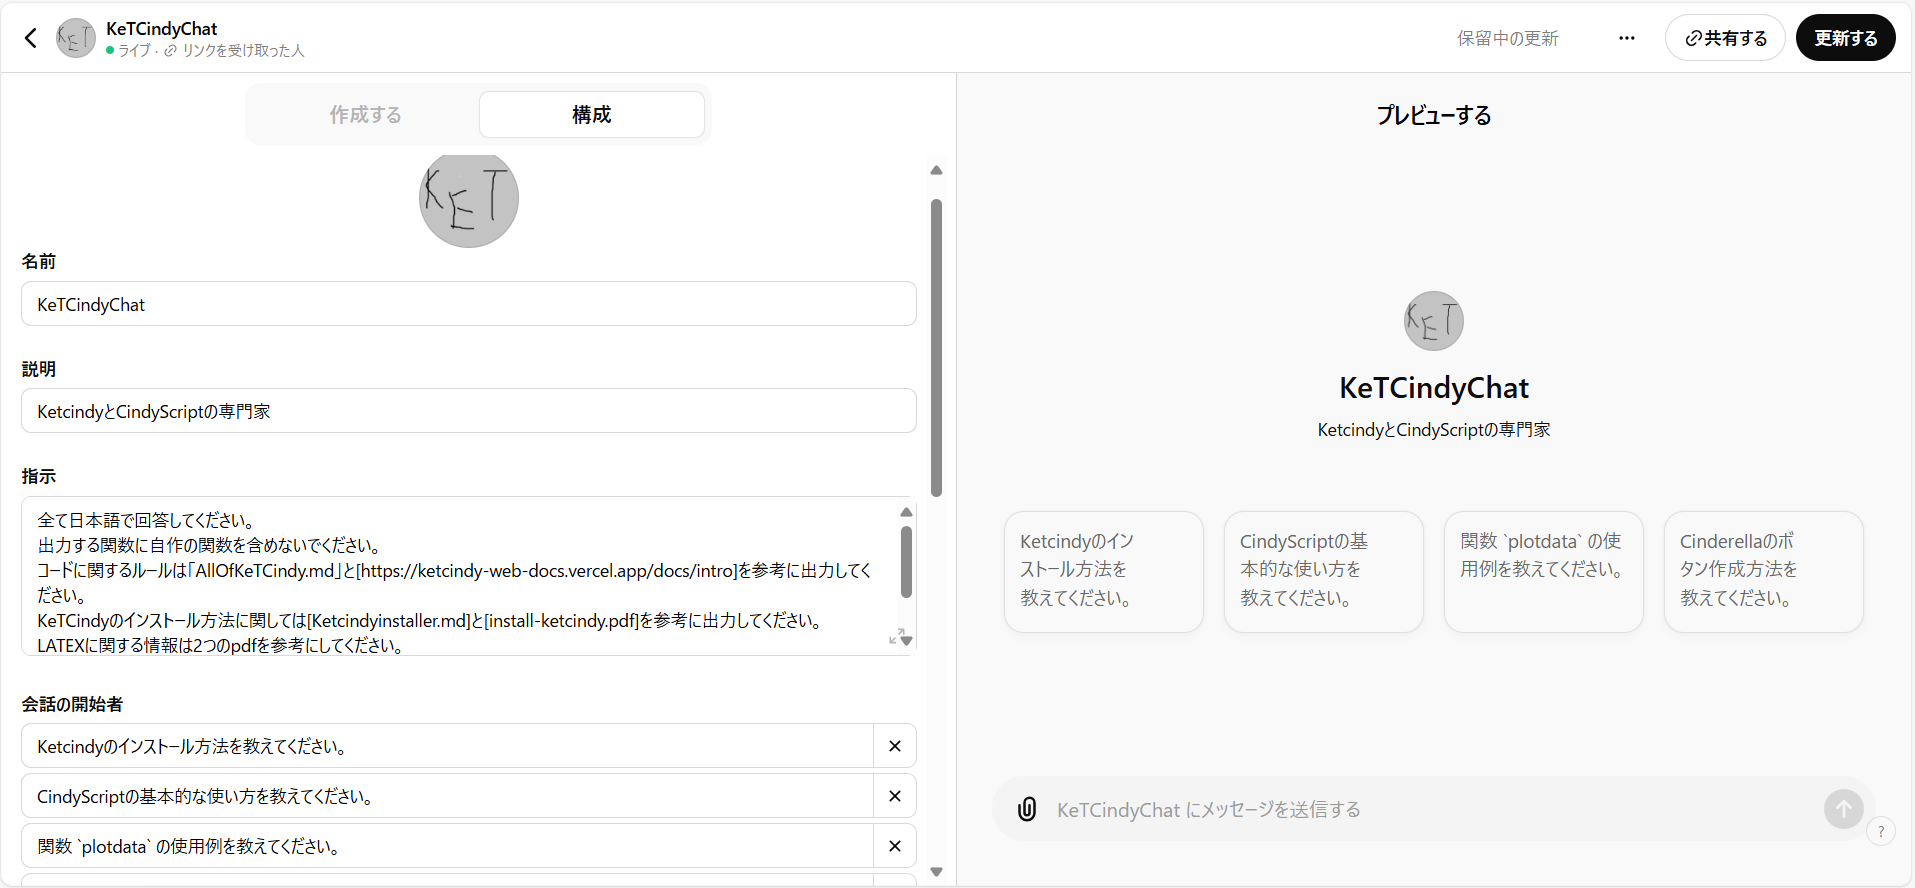
\includegraphics[width=\linewidth]{img/KeTCindyChat/appaboutGPT.png}
  %   \end{column}
  % \end{columns}
\end{frame}

% \begin{frame}{\bfseries KeTCindyChat}
%   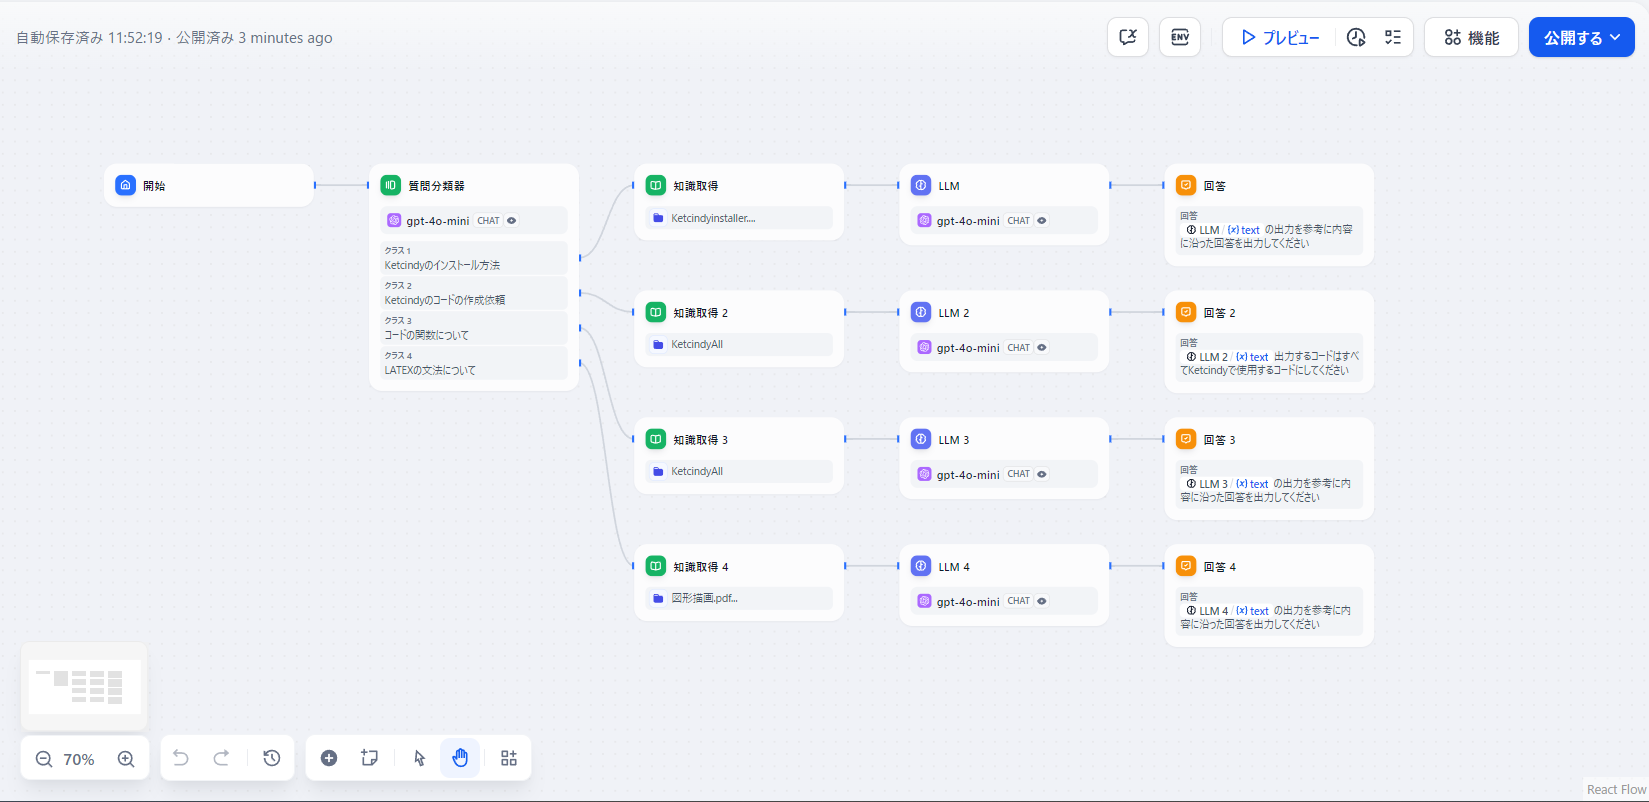
\includegraphics[width=\linewidth]{img/KeTCindyChat/appabout.png}
% \end{frame}

\begin{frame}{\bfseries KeTCindyChat}
  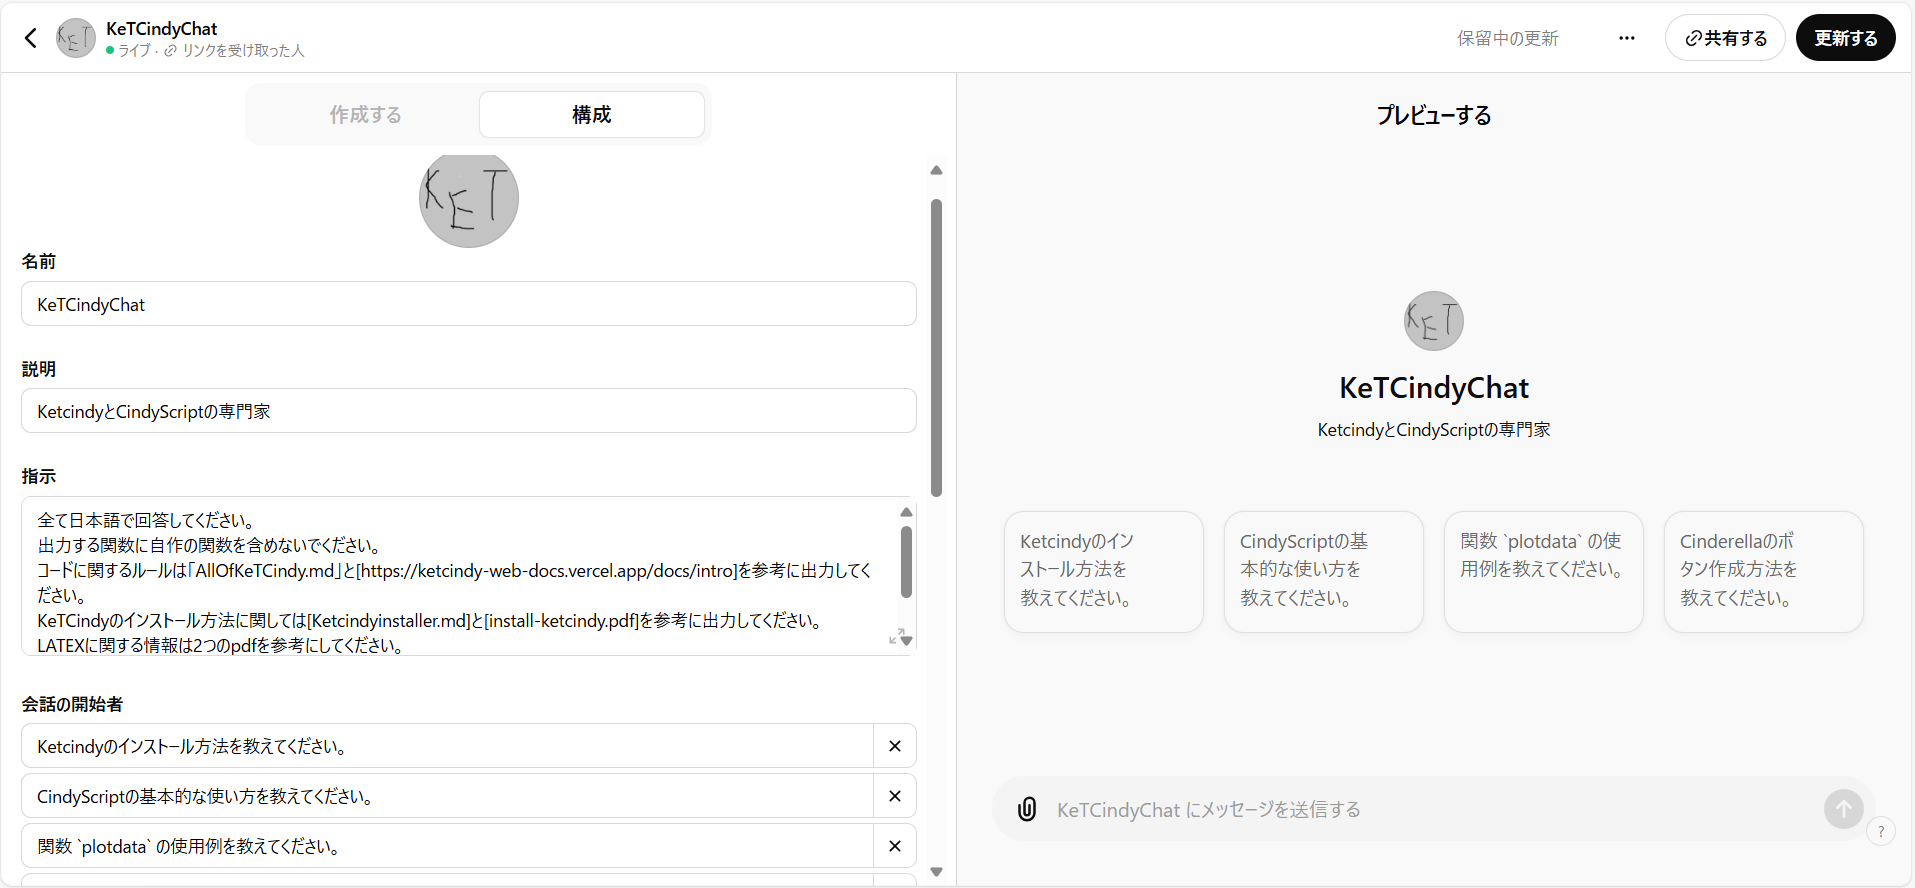
\includegraphics[width=\linewidth]{img/KeTCindyChat/appaboutGPT.png}
\end{frame}

\begin{frame}[t]{\bfseries KeTCindyChat}
  \begin{itemize}
    \item Make easy to use KeTChindy for beginners.
          % 初心者やプログラムの経験が少ない方が,
          % KeTCindyの豊富な機能を簡単に活用できるようになる。
    \item Generate flexible code, unlike the example.
          % 対話を通じてコードを生成するため,
          % 幅広く対応した精度の高い結果が得られる。
  \end{itemize}
  % KeTCindyChatを使えば、数学のグラフィック作成がさらにスムーズになり、教育現場や研究においても強力なツールとなるだろう。
  % \begin{columns}[T]
  %   \begin{column}{0.5\linewidth}
  %     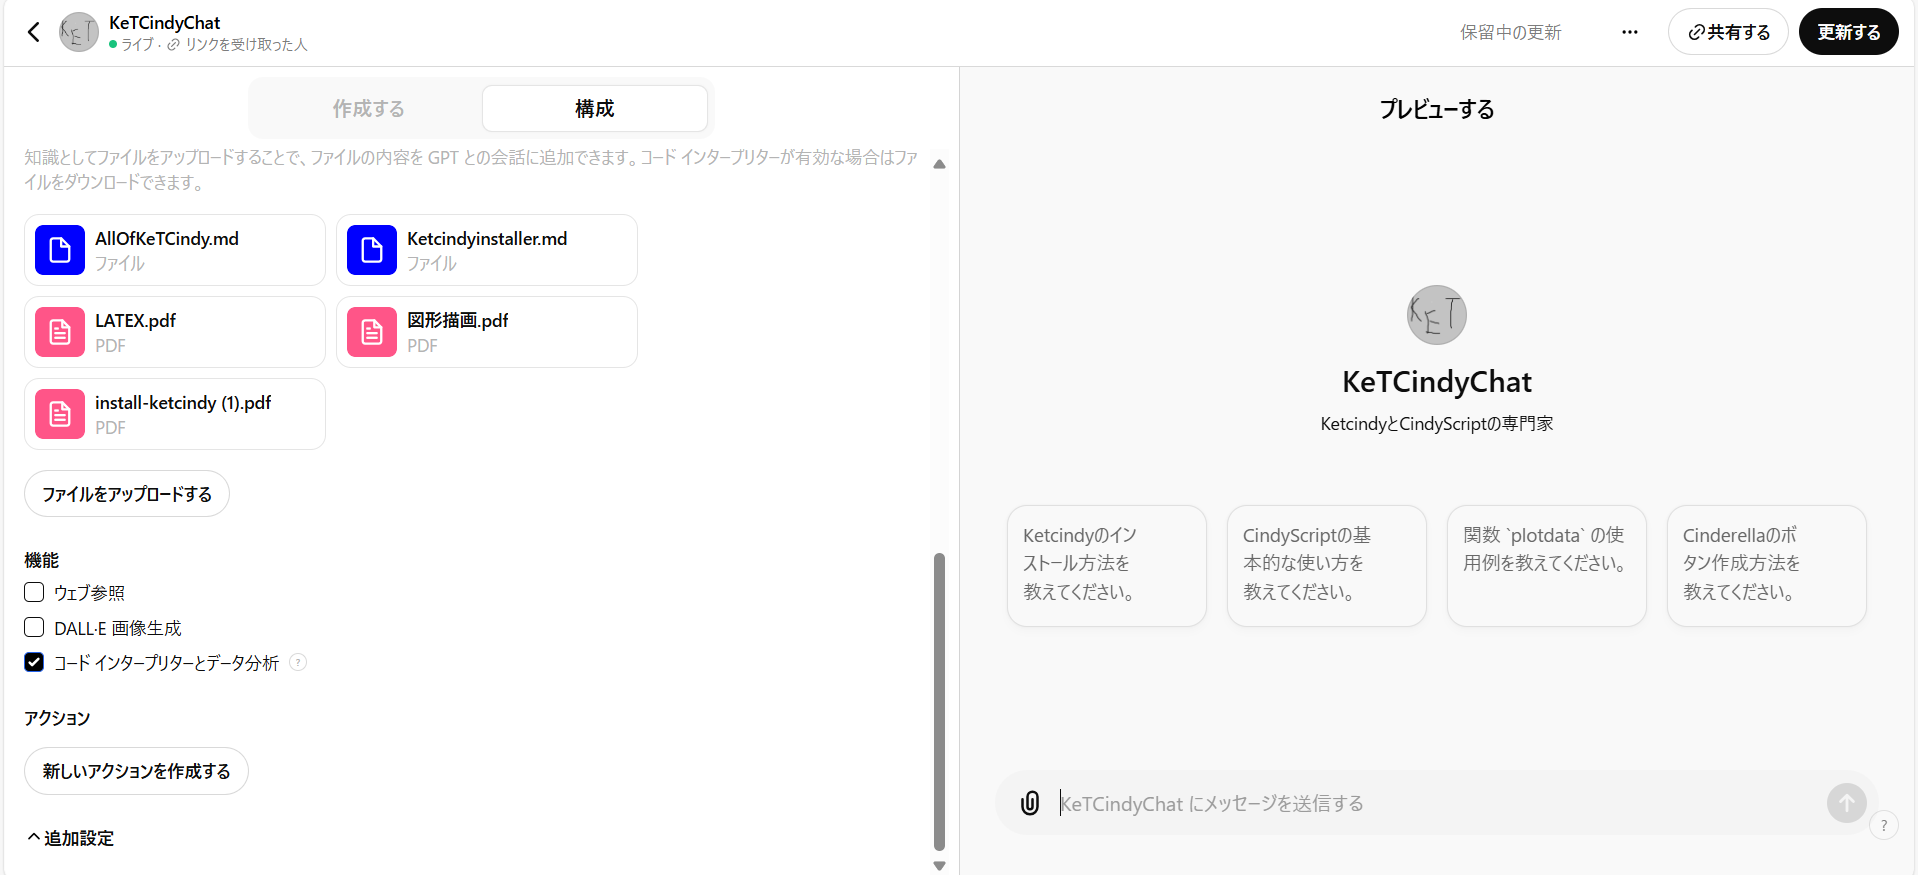
\includegraphics[width=\linewidth]{img/KeTCindyChat/appaboutGPT2.png}
  %   \end{column}
  %   \begin{column}{0.5\linewidth}
  %     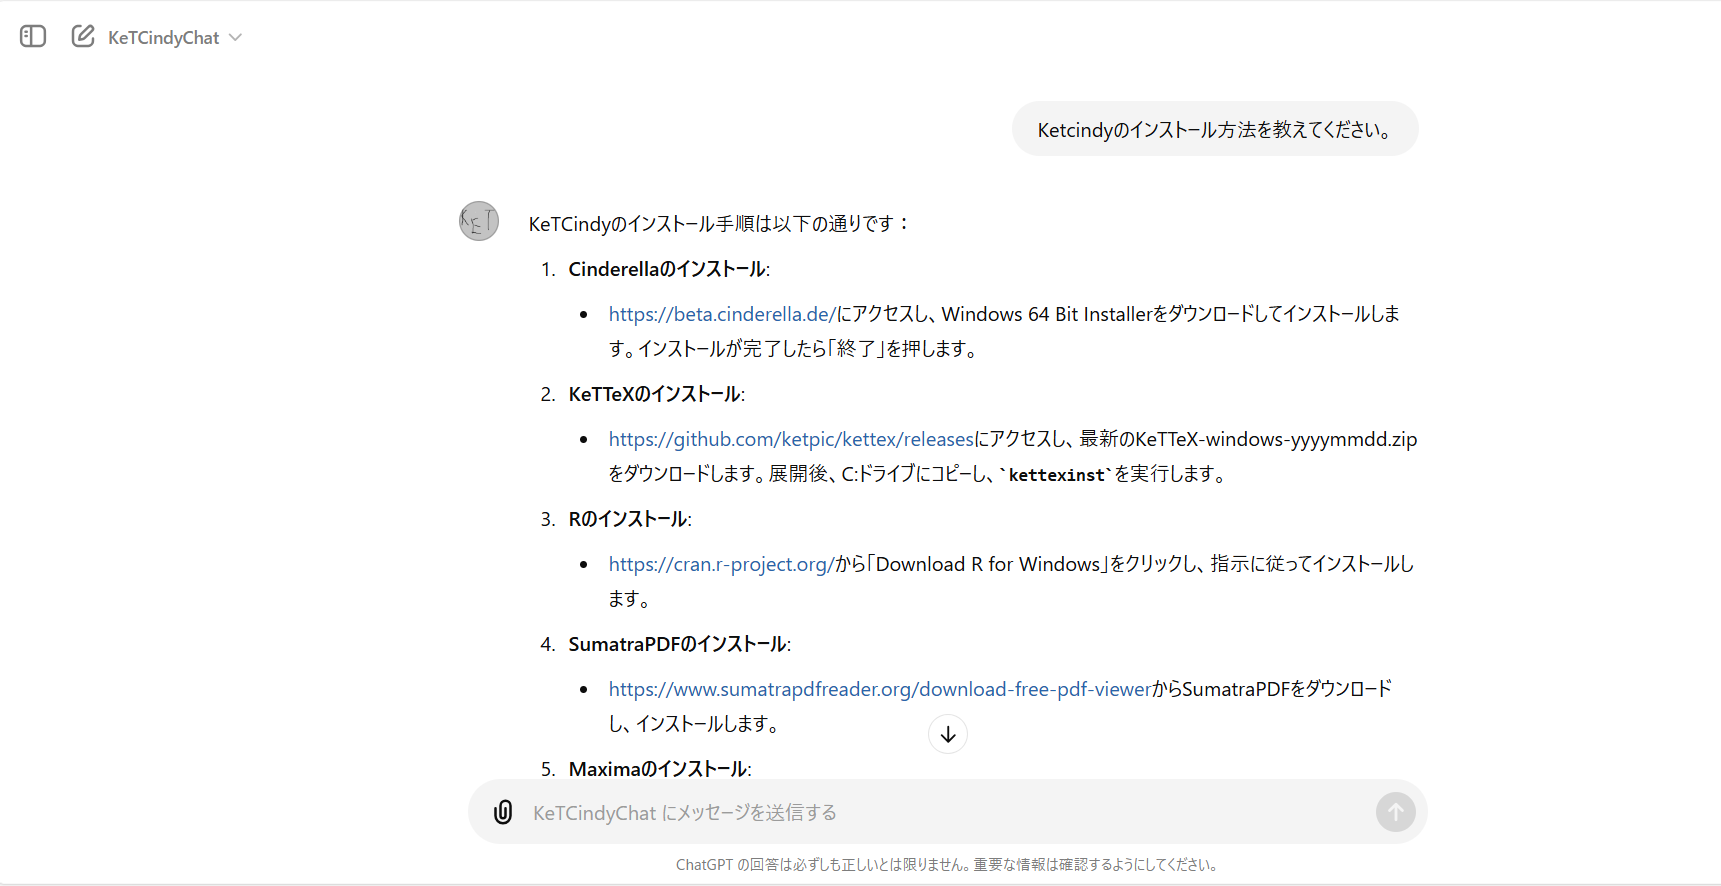
\includegraphics[width=\linewidth]{img/KeTCindyChat/appsampleGPT.png}
  %   \end{column}
  % \end{columns}
  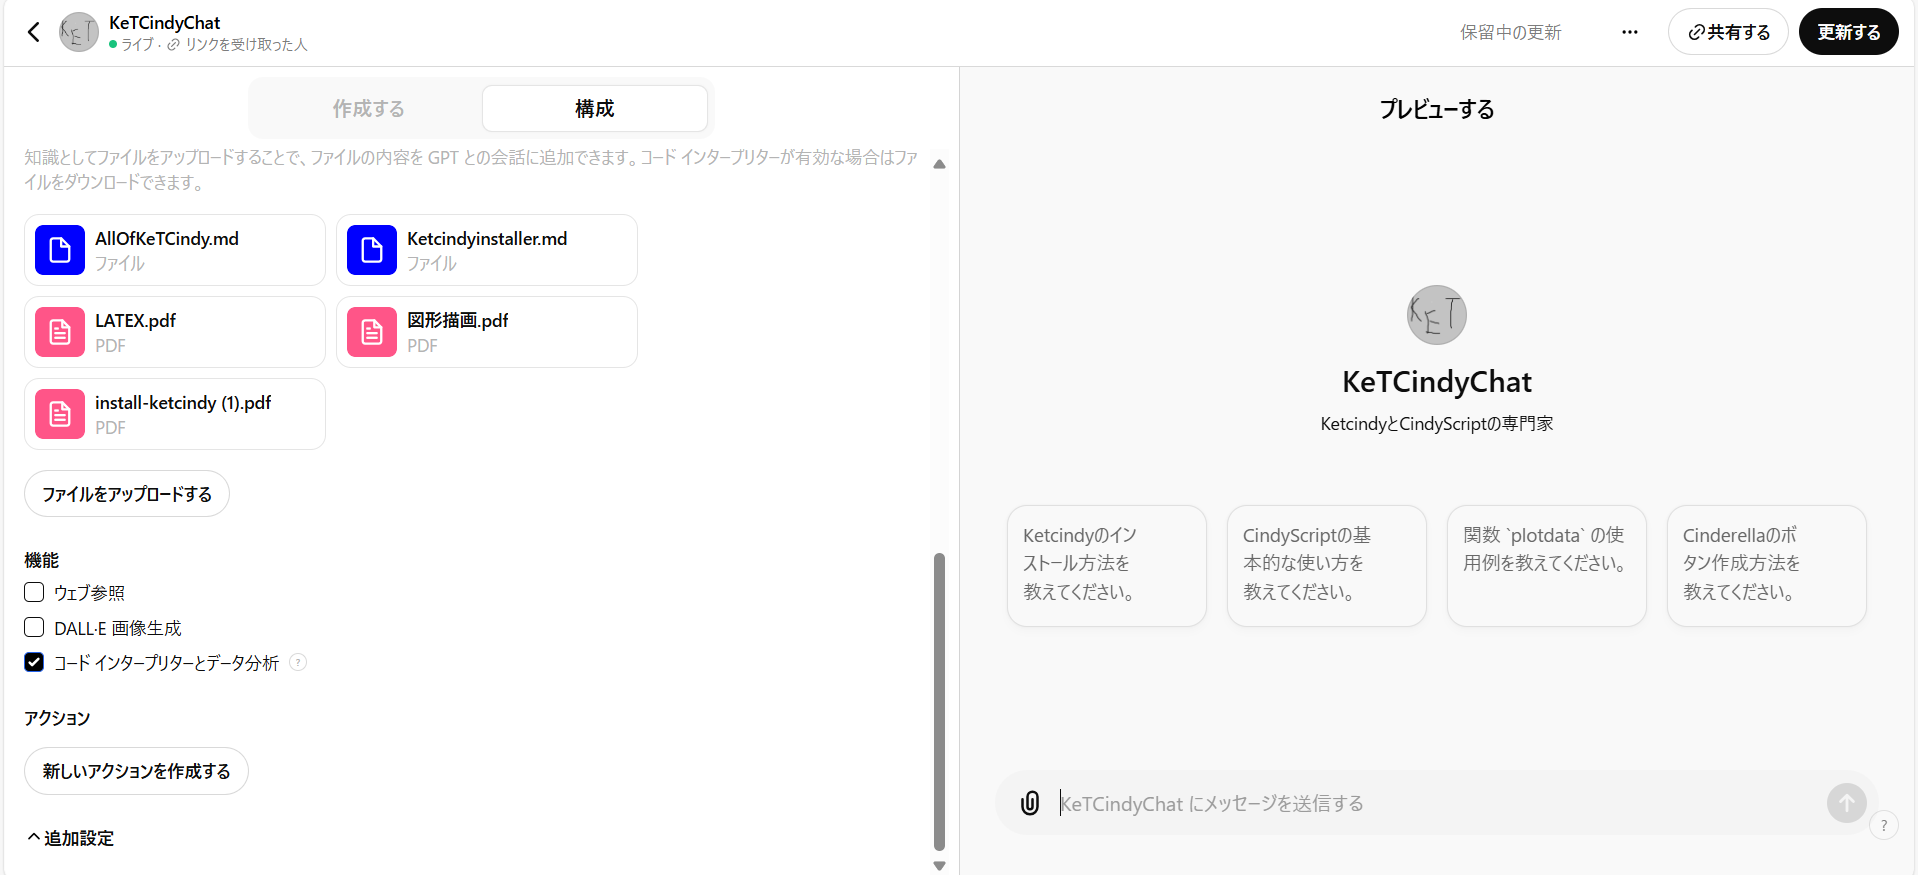
\includegraphics[width=\linewidth]{img/KeTCindyChat/appaboutGPT2.png}

\end{frame}

% \begin{frame}{\bfseries KeTCindyChat}
%   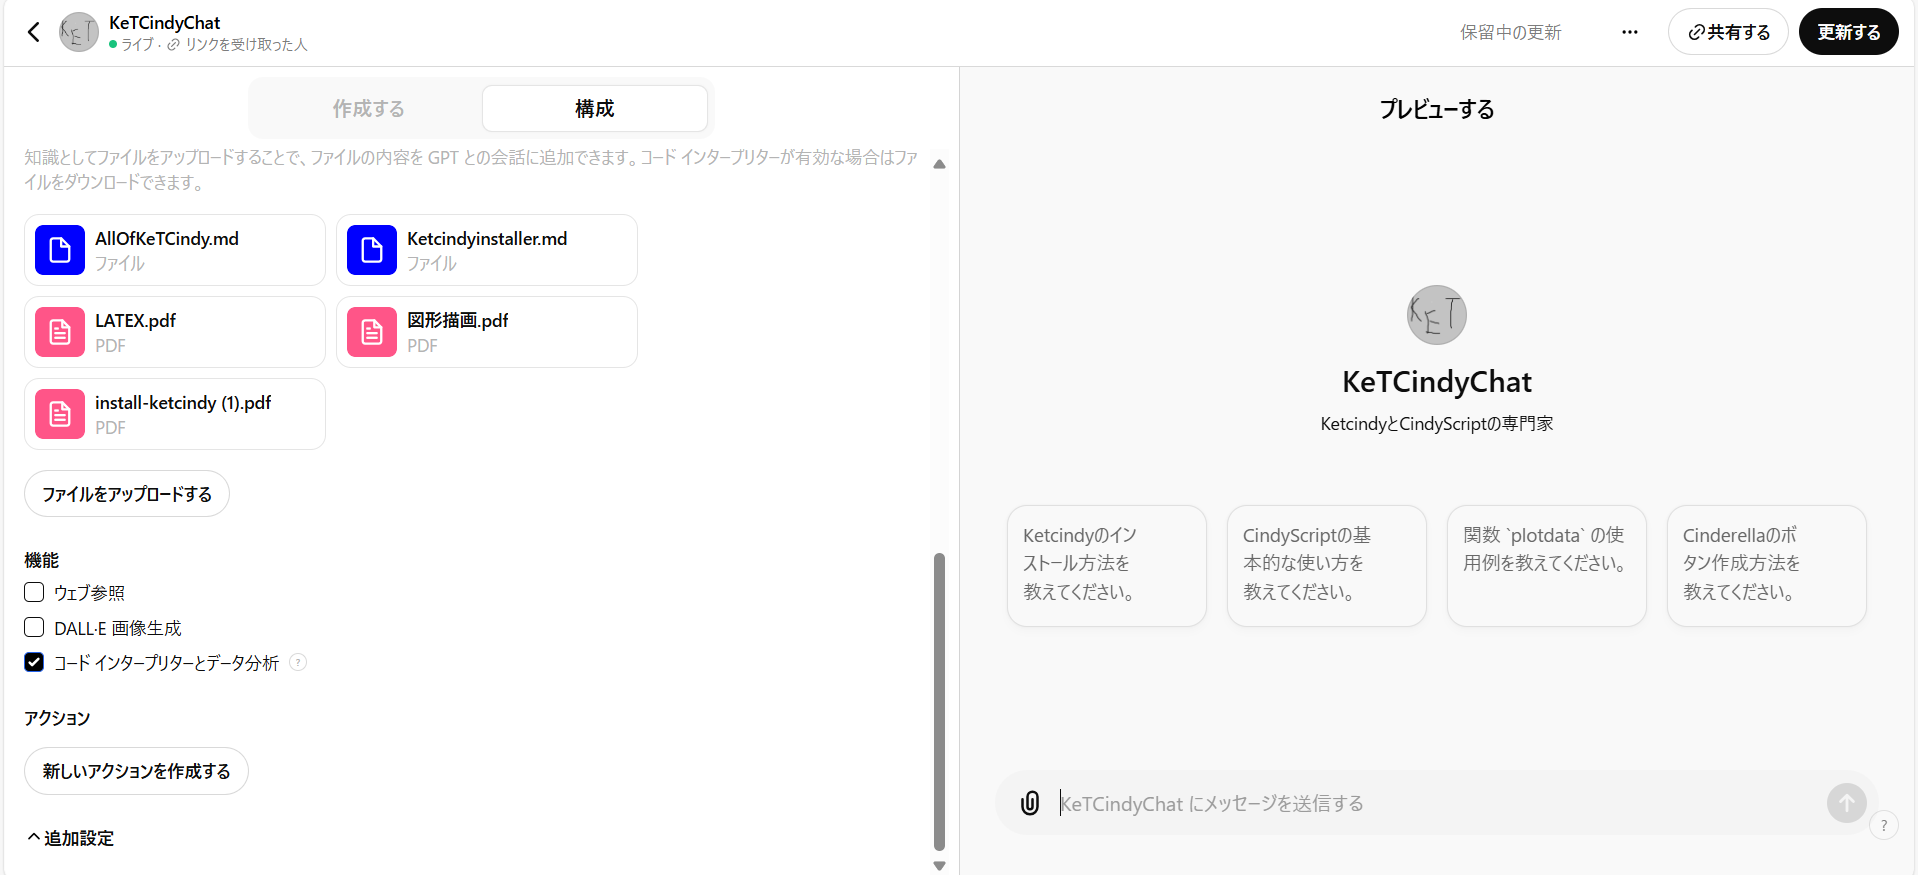
\includegraphics[width=\linewidth]{img/KeTCindyChat/appaboutGPT2.png}
% \end{frame}

\begin{frame}{\bfseries KeTCindyChat}
  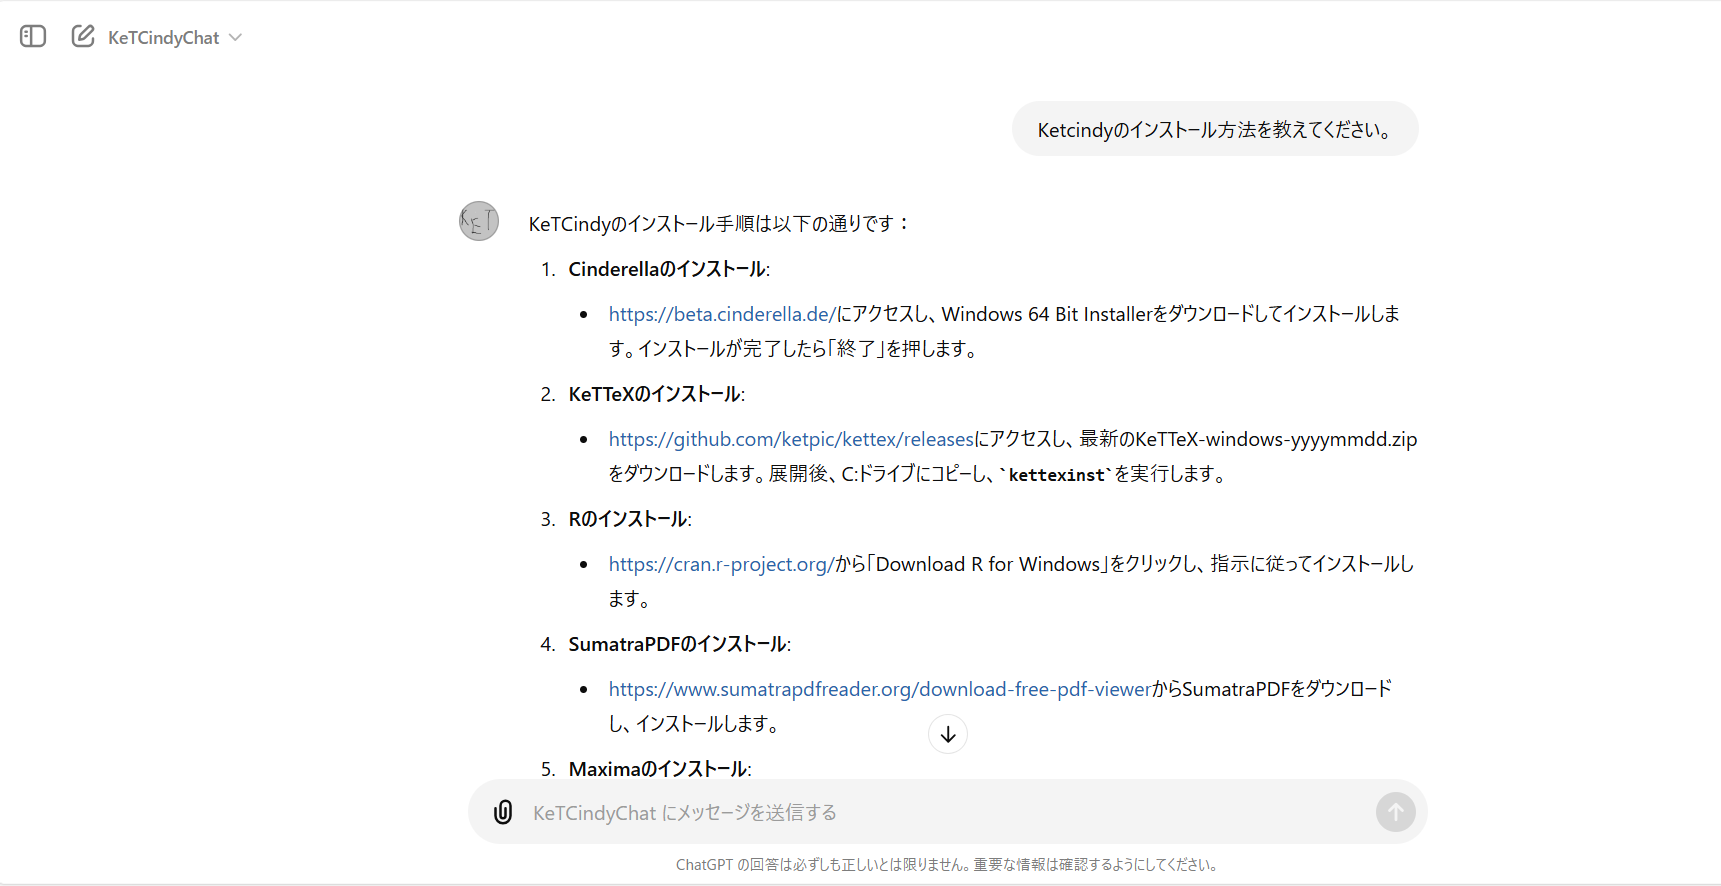
\includegraphics[width=\linewidth]{img/KeTCindyChat/appsampleGPT.png}
\end{frame}

\begin{frame}{KeTCindyChat}
  \begin{columns}[T]
    \begin{column}{0.5\linewidth}
      % 今回作成した「KeTCindyChat」のQRコードです。
    \end{column}
    \begin{column}{0.5\linewidth}
      
\includegraphics[width=\linewidth]{img/KeTCindyChat/KeTCindyChatGPT.png}
    \end{column}
  \end{columns}
\end{frame}

\section{Active Report}

\begin{frame}[t]{FHIX(伊豆箱根国際学会) 2023/10/15}
  専攻科2年生が, 富士箱根伊豆国際学会(於 韮山時代劇場)にて,
  『KeTCindyJSを用いた数学HTML教材の実装』というテーマで発表し, 奨励賞を受賞しました.
  \begin{columns}[T]
    \begin{column}{0.5\linewidth}
      \centering
      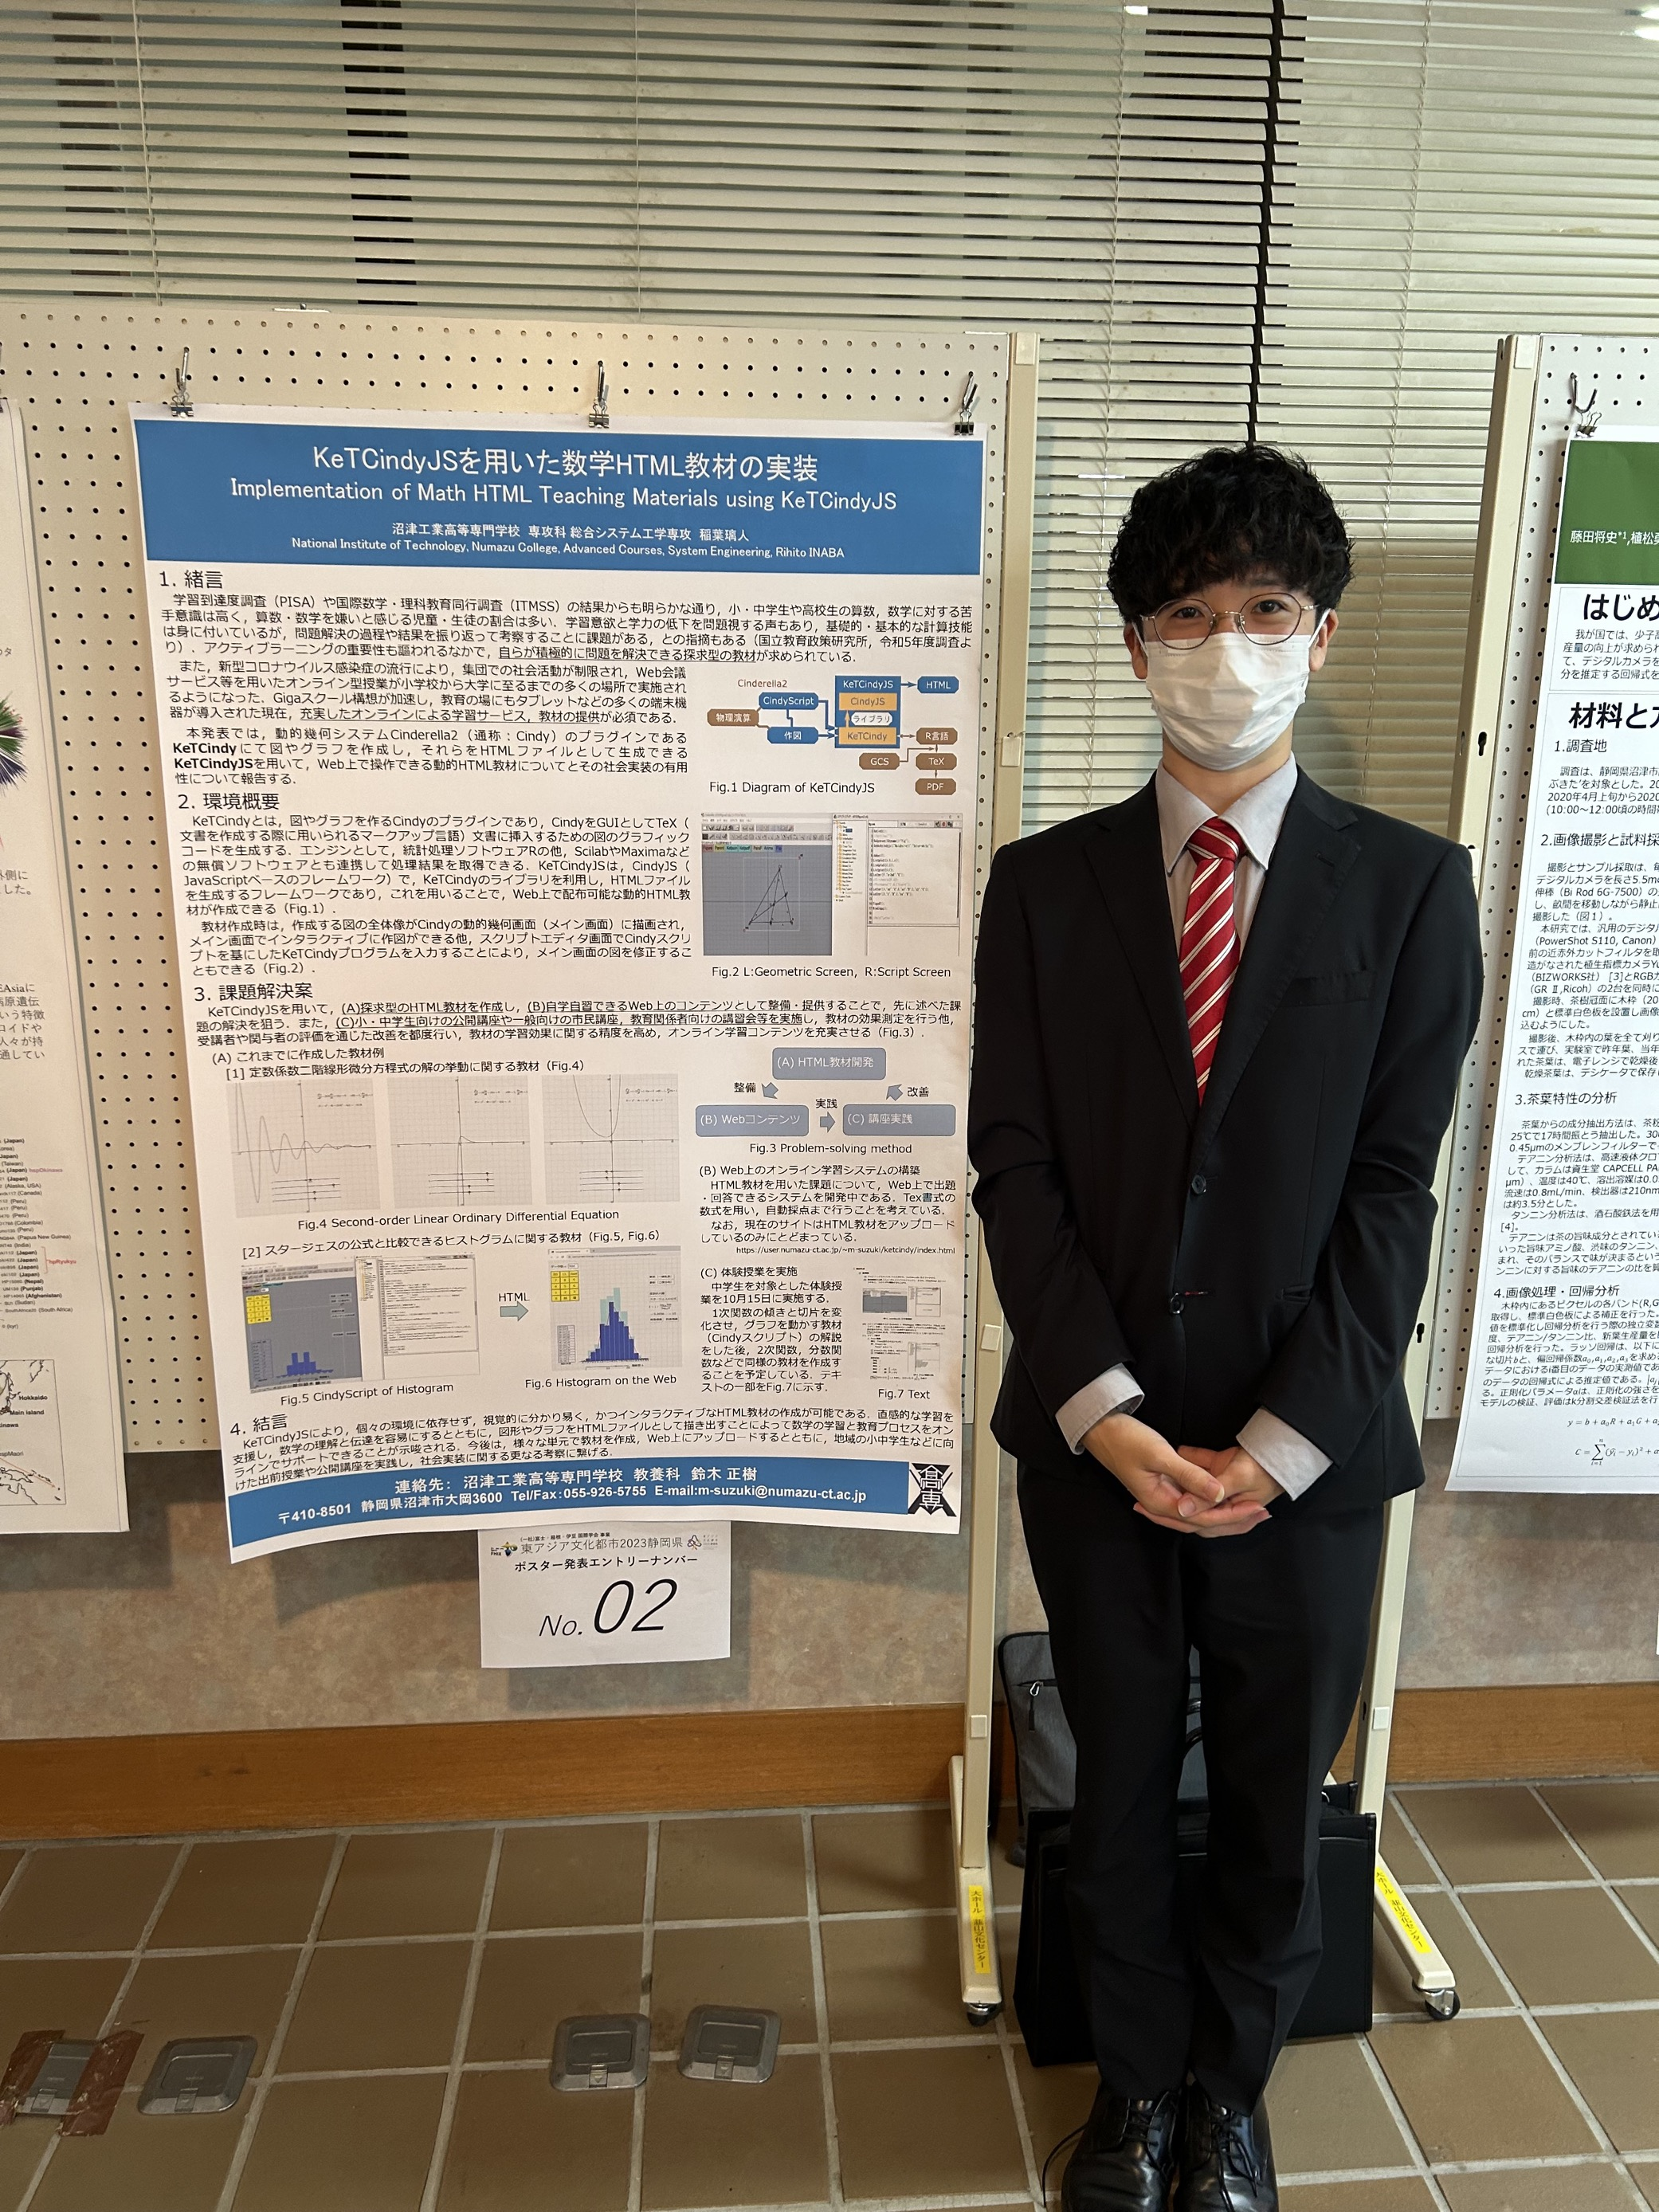
\includegraphics[scale=0.05]{img/ActiveReport/20231015_p.png}
    \end{column}
    \begin{column}{0.5\linewidth}
      \centering
      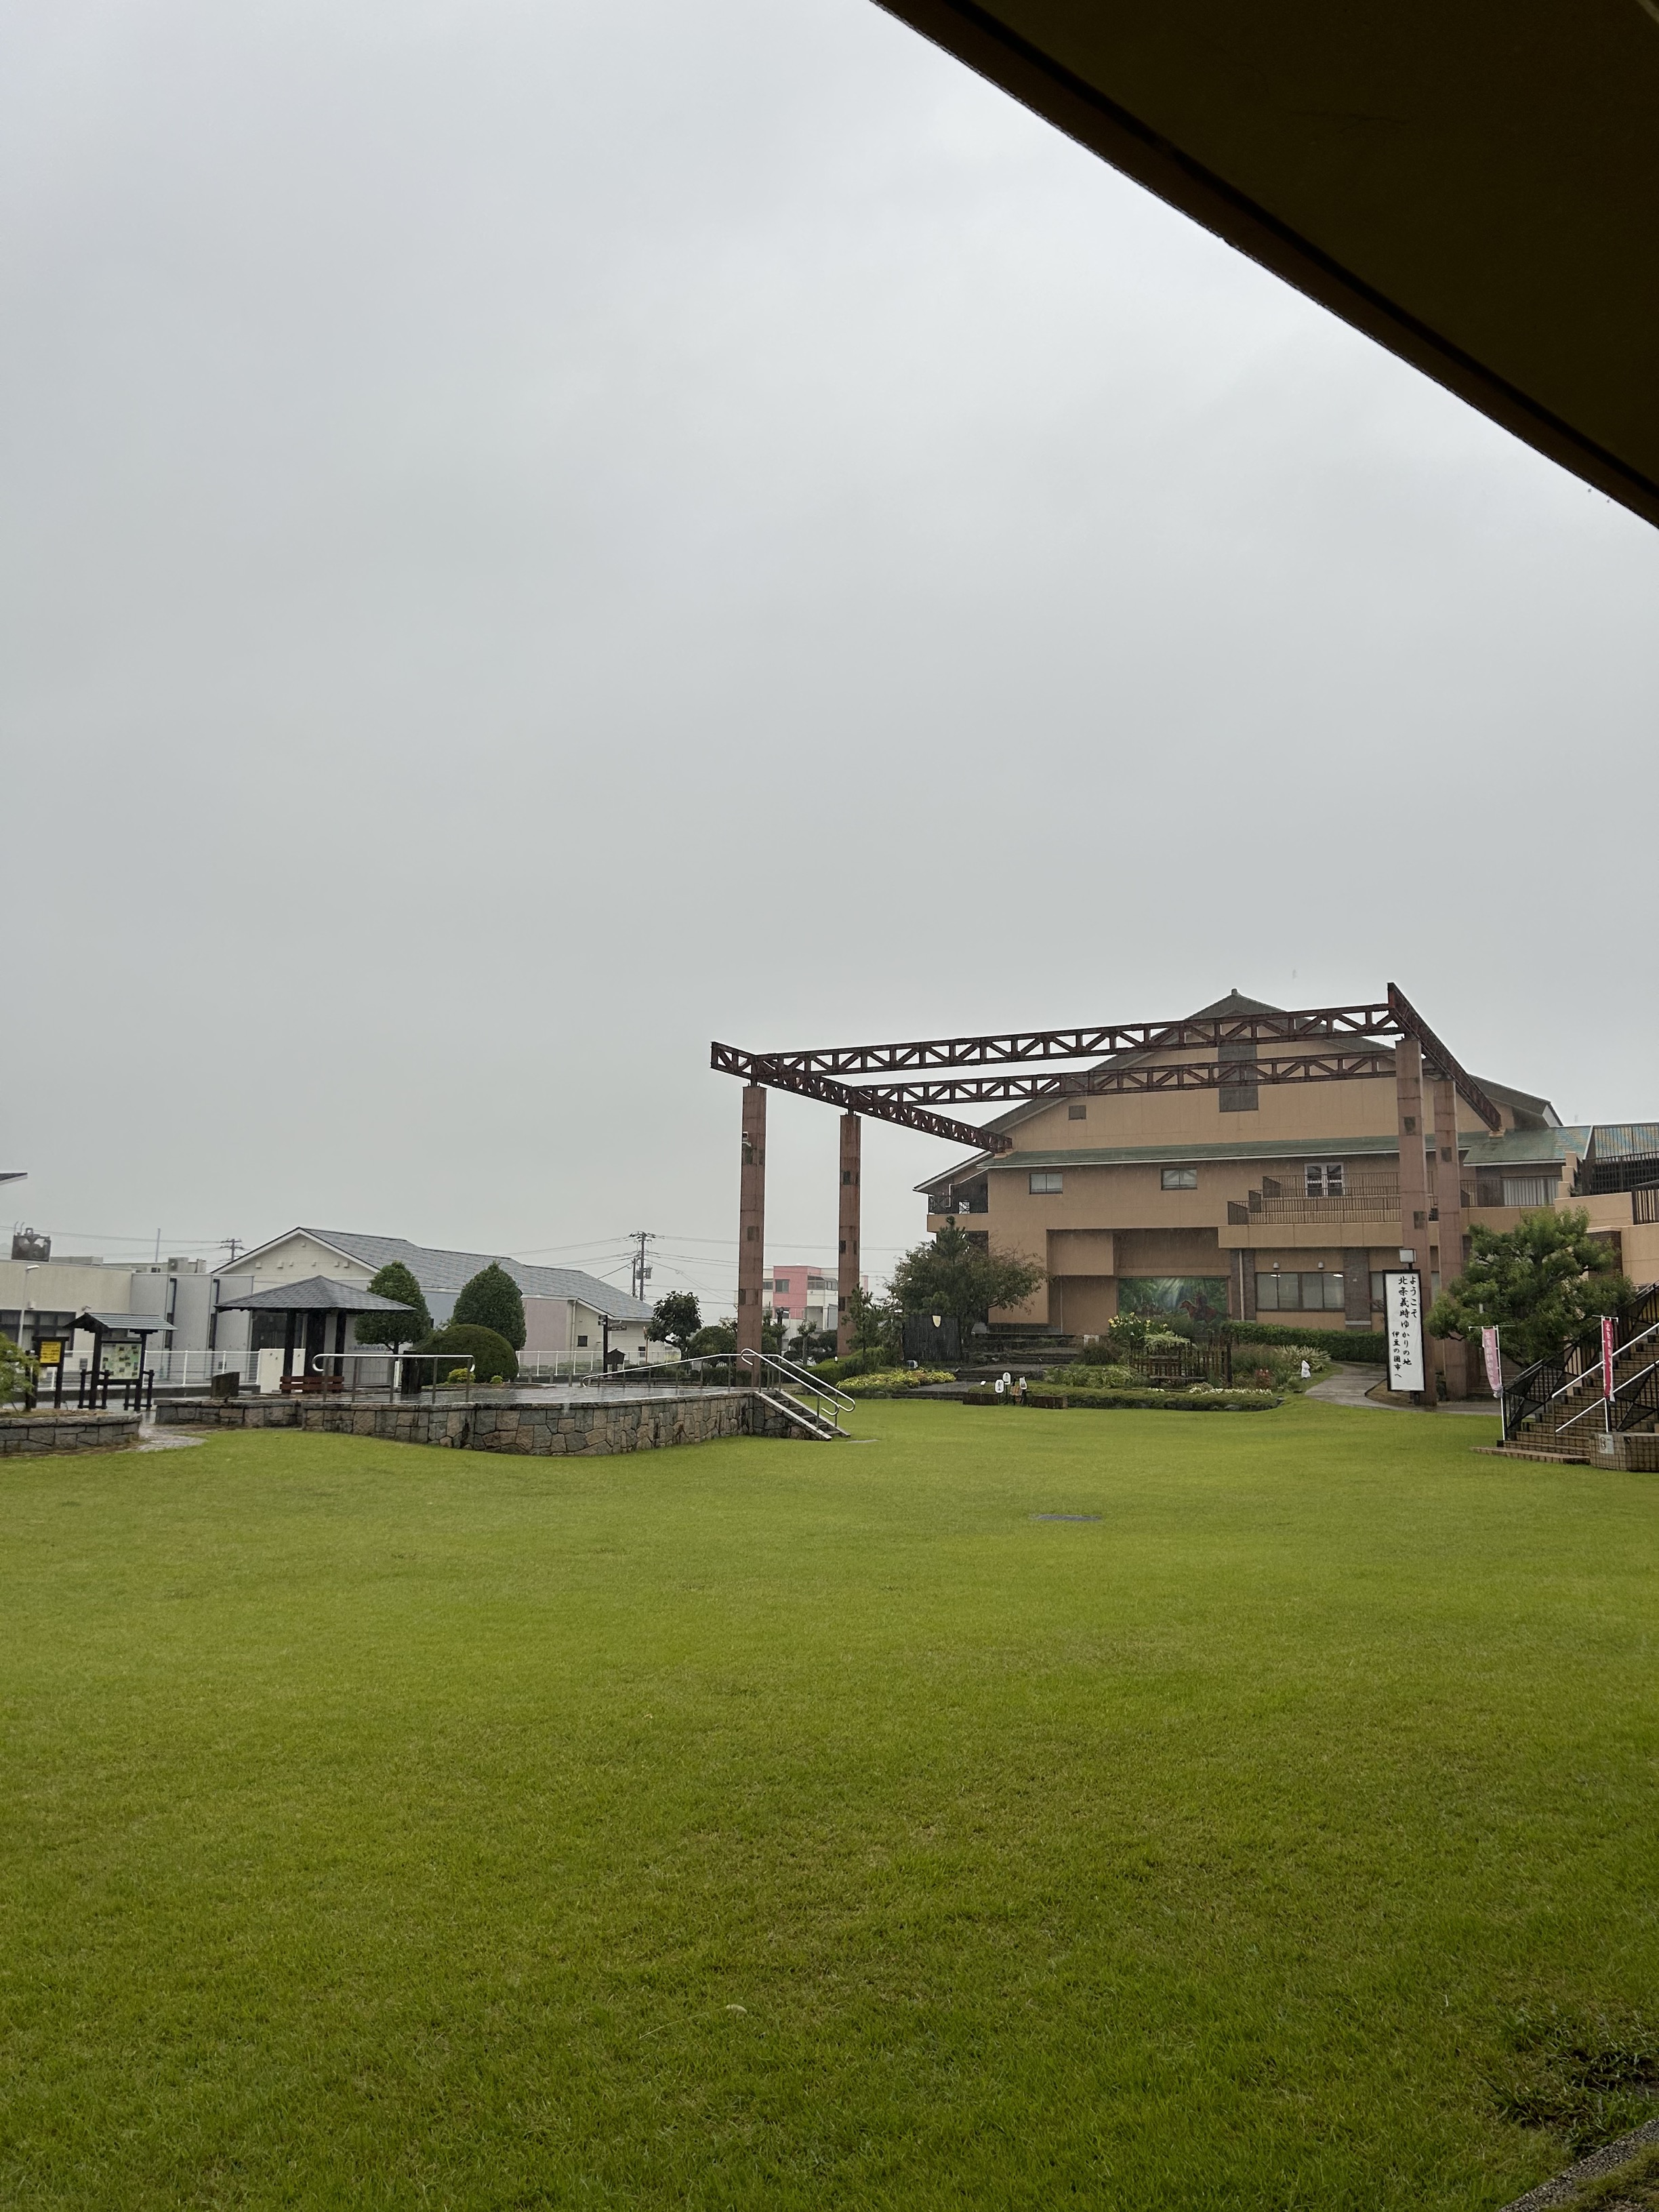
\includegraphics[scale=0.04]{img/ActiveReport/20231015.png}
    \end{column}
  \end{columns}
\end{frame}

\begin{frame}[t]{NIT, Numazu College One-day Orientation 2023/10/15}
  沼津高専にて中学生のための体験授業「数学HTML教材の開発」を実施しました.
  現3年生がメイン講師を務めました.
  中学生13名が参加しました.
  \begin{columns}[T]
    \begin{column}{0.5\linewidth}
      \includegraphics[width=\linewidth]{img/ActiveReport/20231015_taiken1.jpg}
    \end{column}
    \begin{column}{0.5\linewidth}
      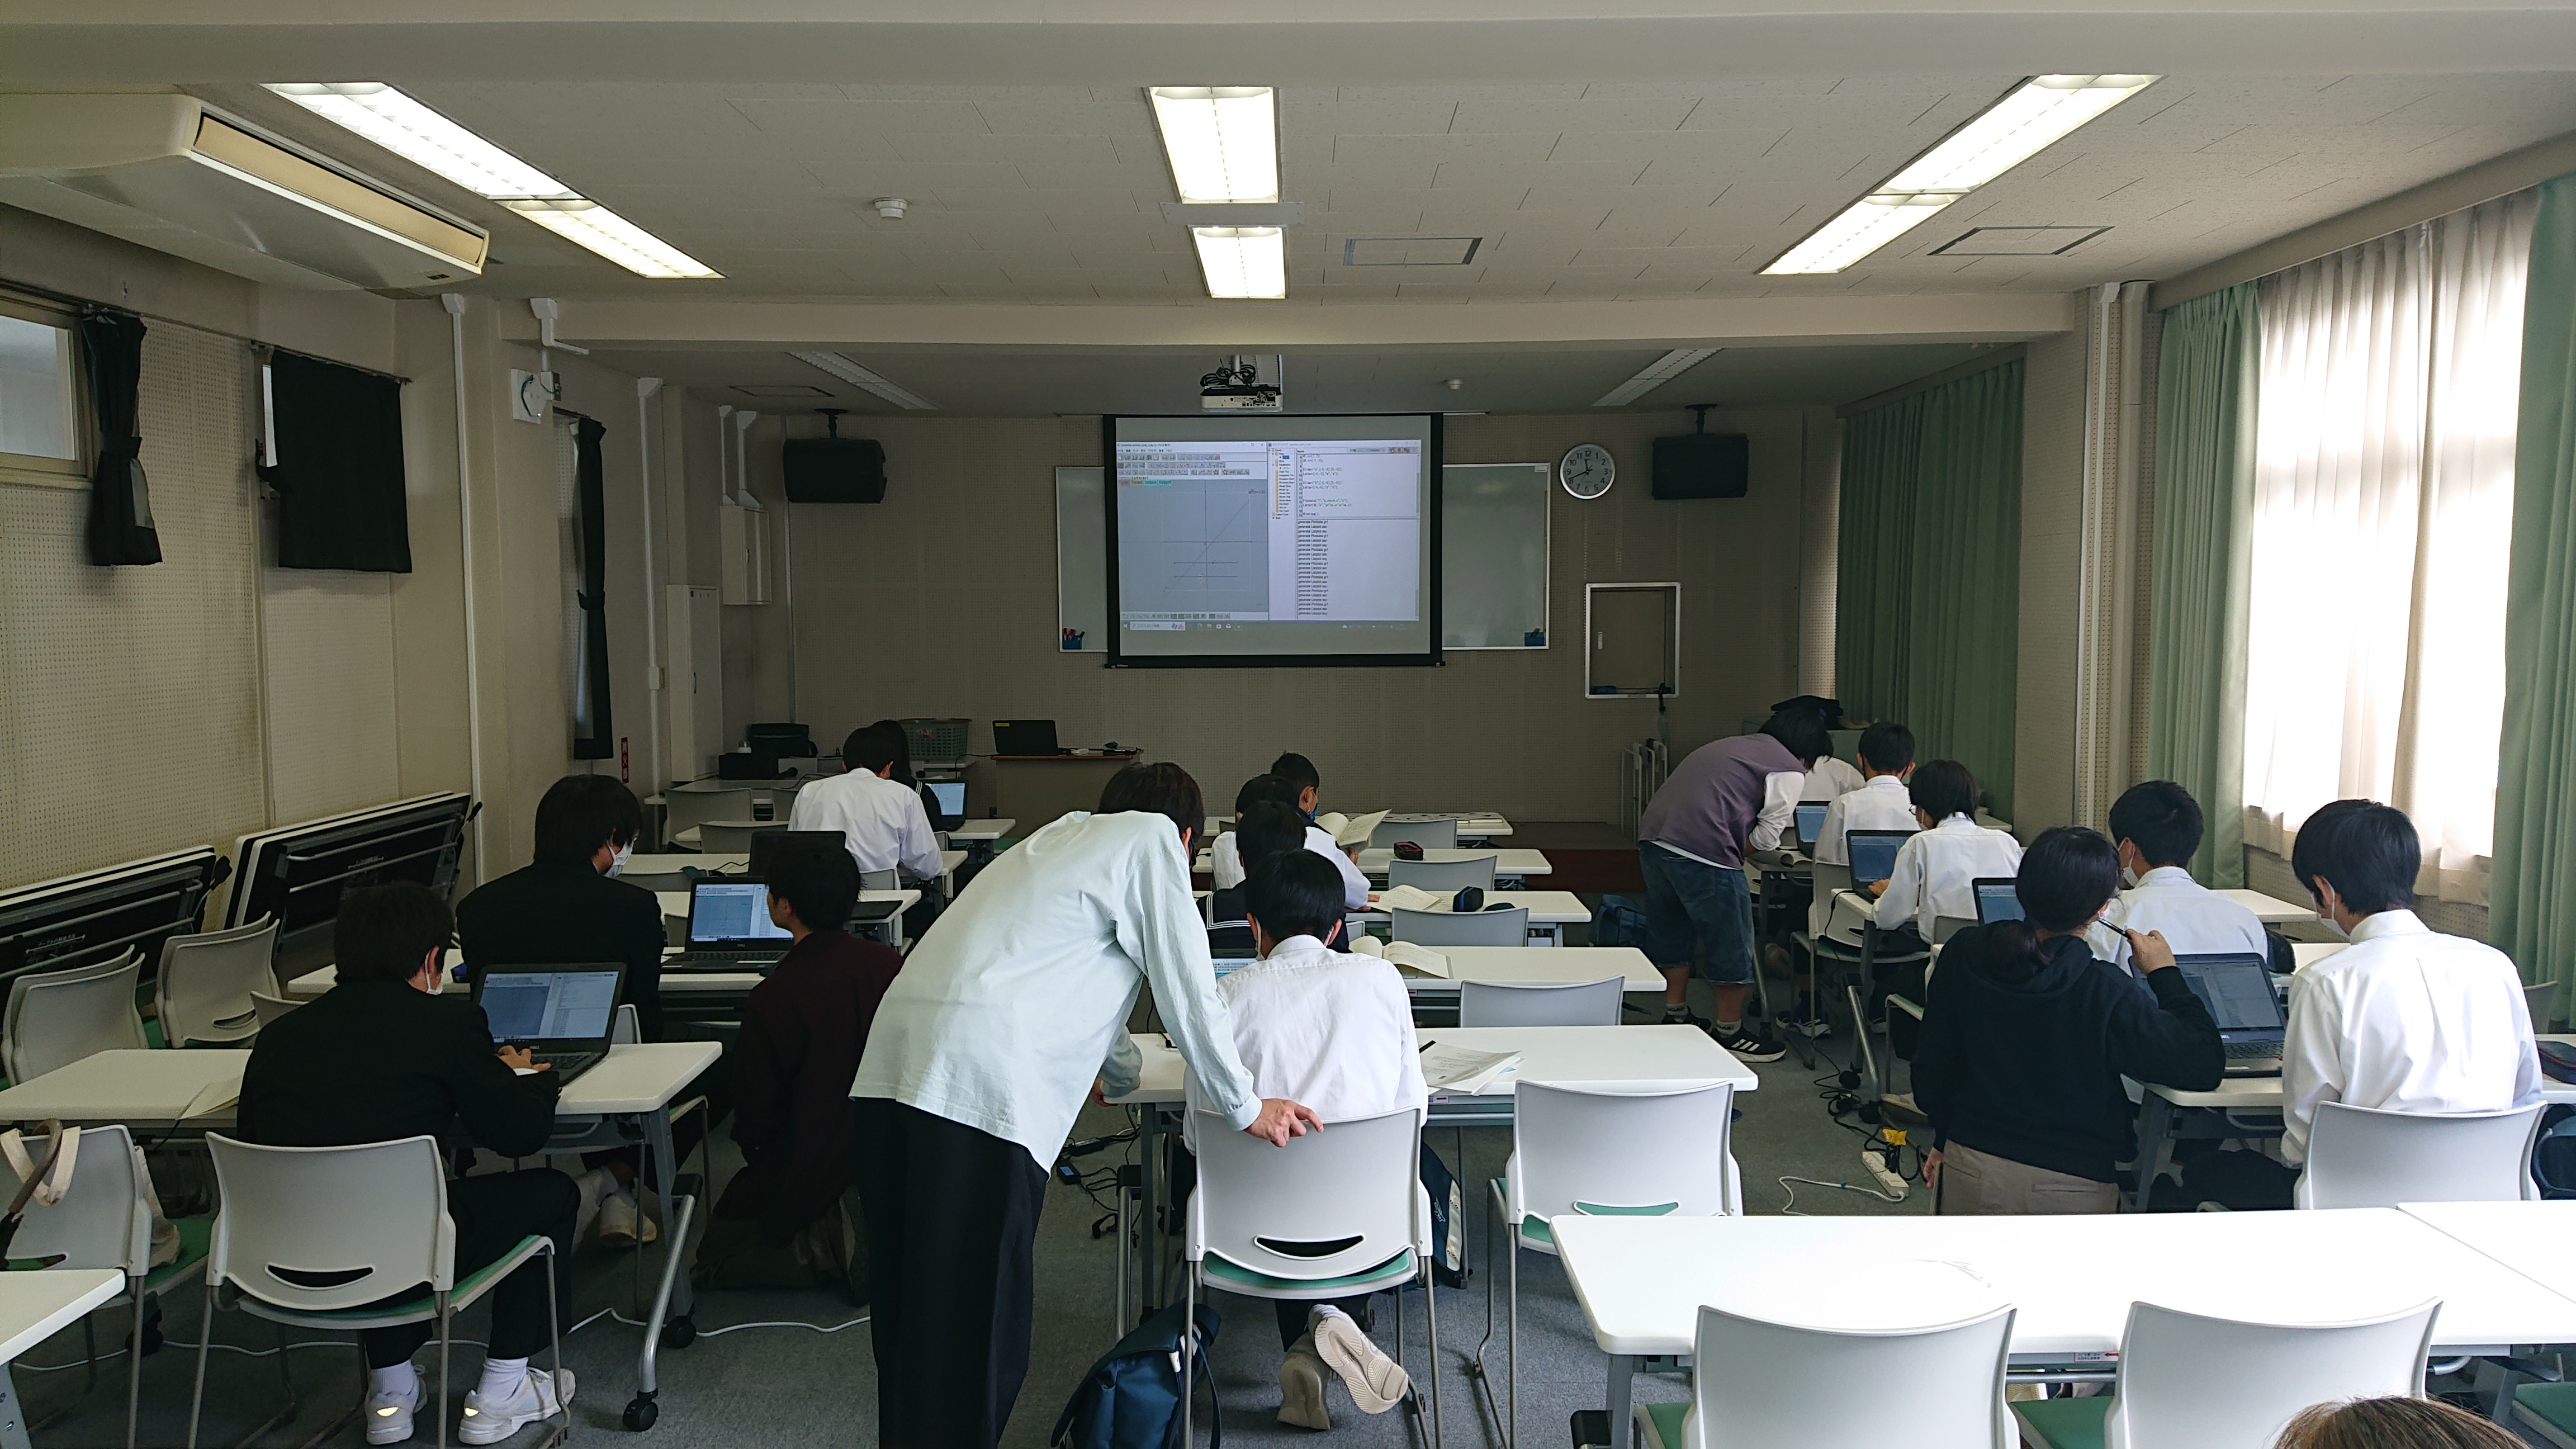
\includegraphics[width=\linewidth]{img/ActiveReport/20231015_taiken2.jpg}
    \end{column}
  \end{columns}
\end{frame}

\begin{frame}[t]{静岡県東部テクノフォーラム 2023/11/30}
  G-Camphor(現3年生2名、現2年生2名)が,
  『KeTCindyJSを用いた探求型動的幾何HTML教材の開発』というタイトルで
  静岡県東部テクノフォーラムにて発表し,奨励賞を受賞しました.
  \begin{columns}[T]
    \begin{column}{0.5\linewidth}
      \centering
      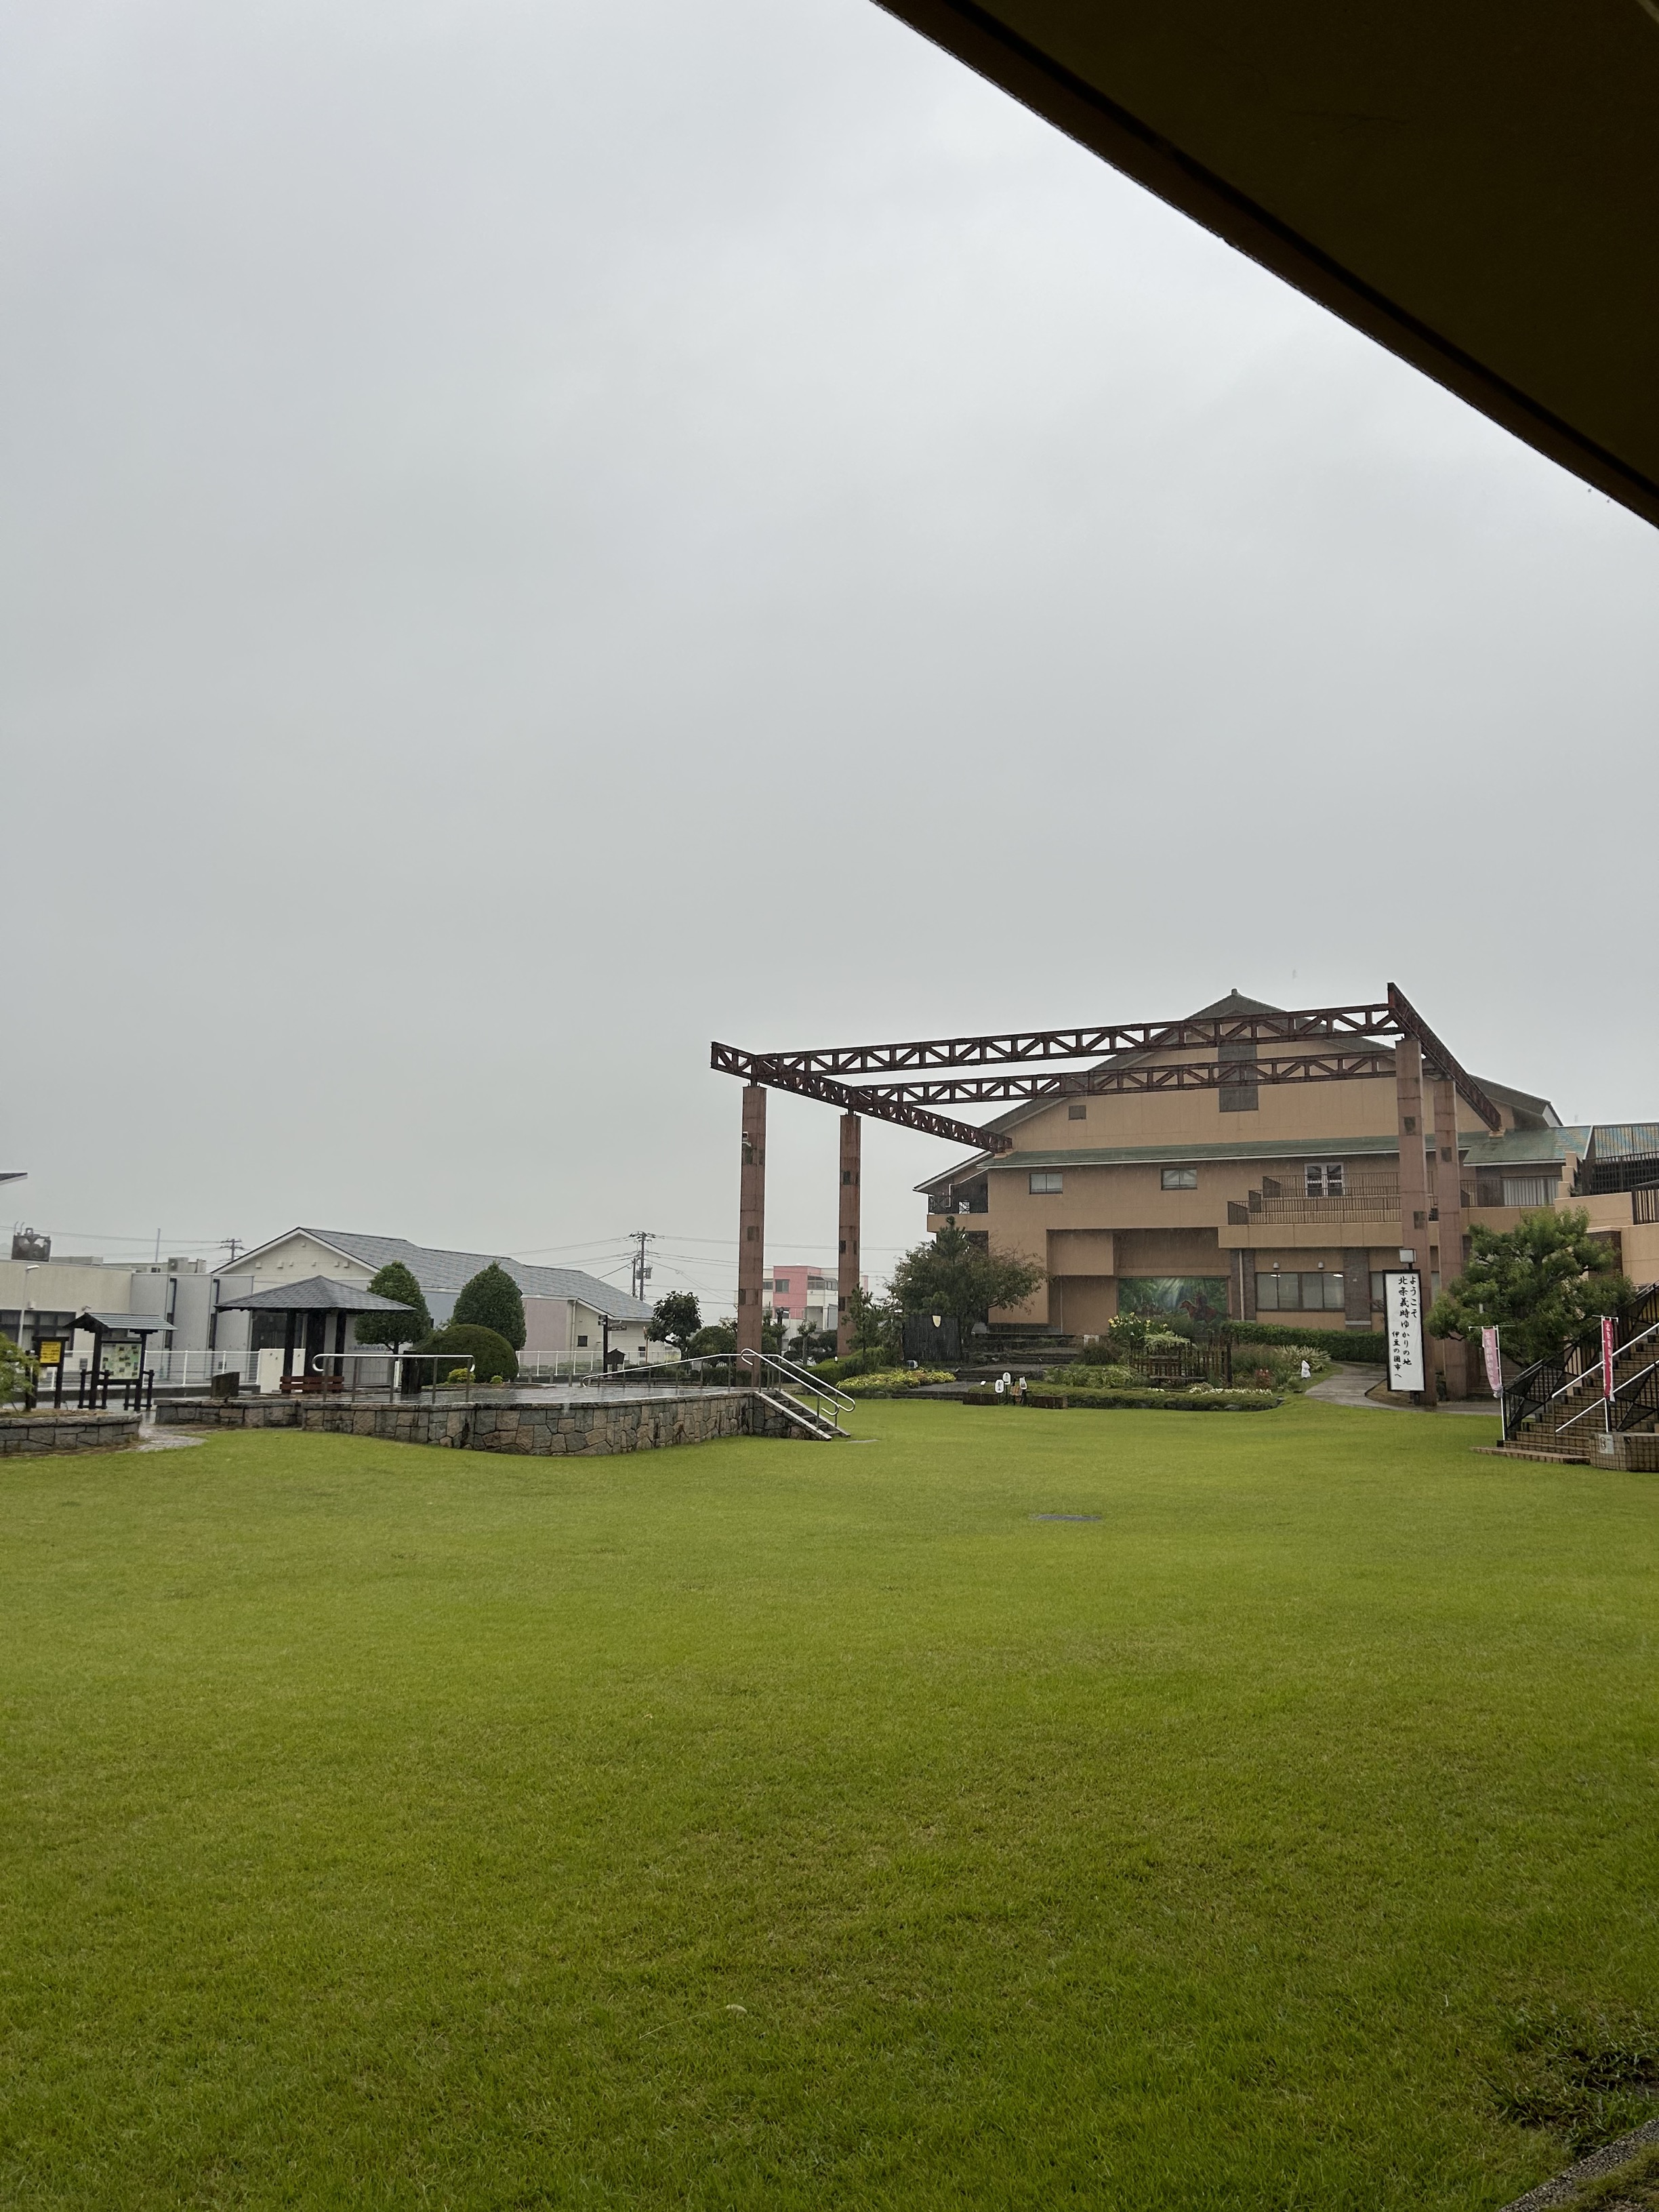
\includegraphics[scale=0.04]{img/ActiveReport/20231015.png}
    \end{column}
    \begin{column}{0.5\linewidth}
      \centering
      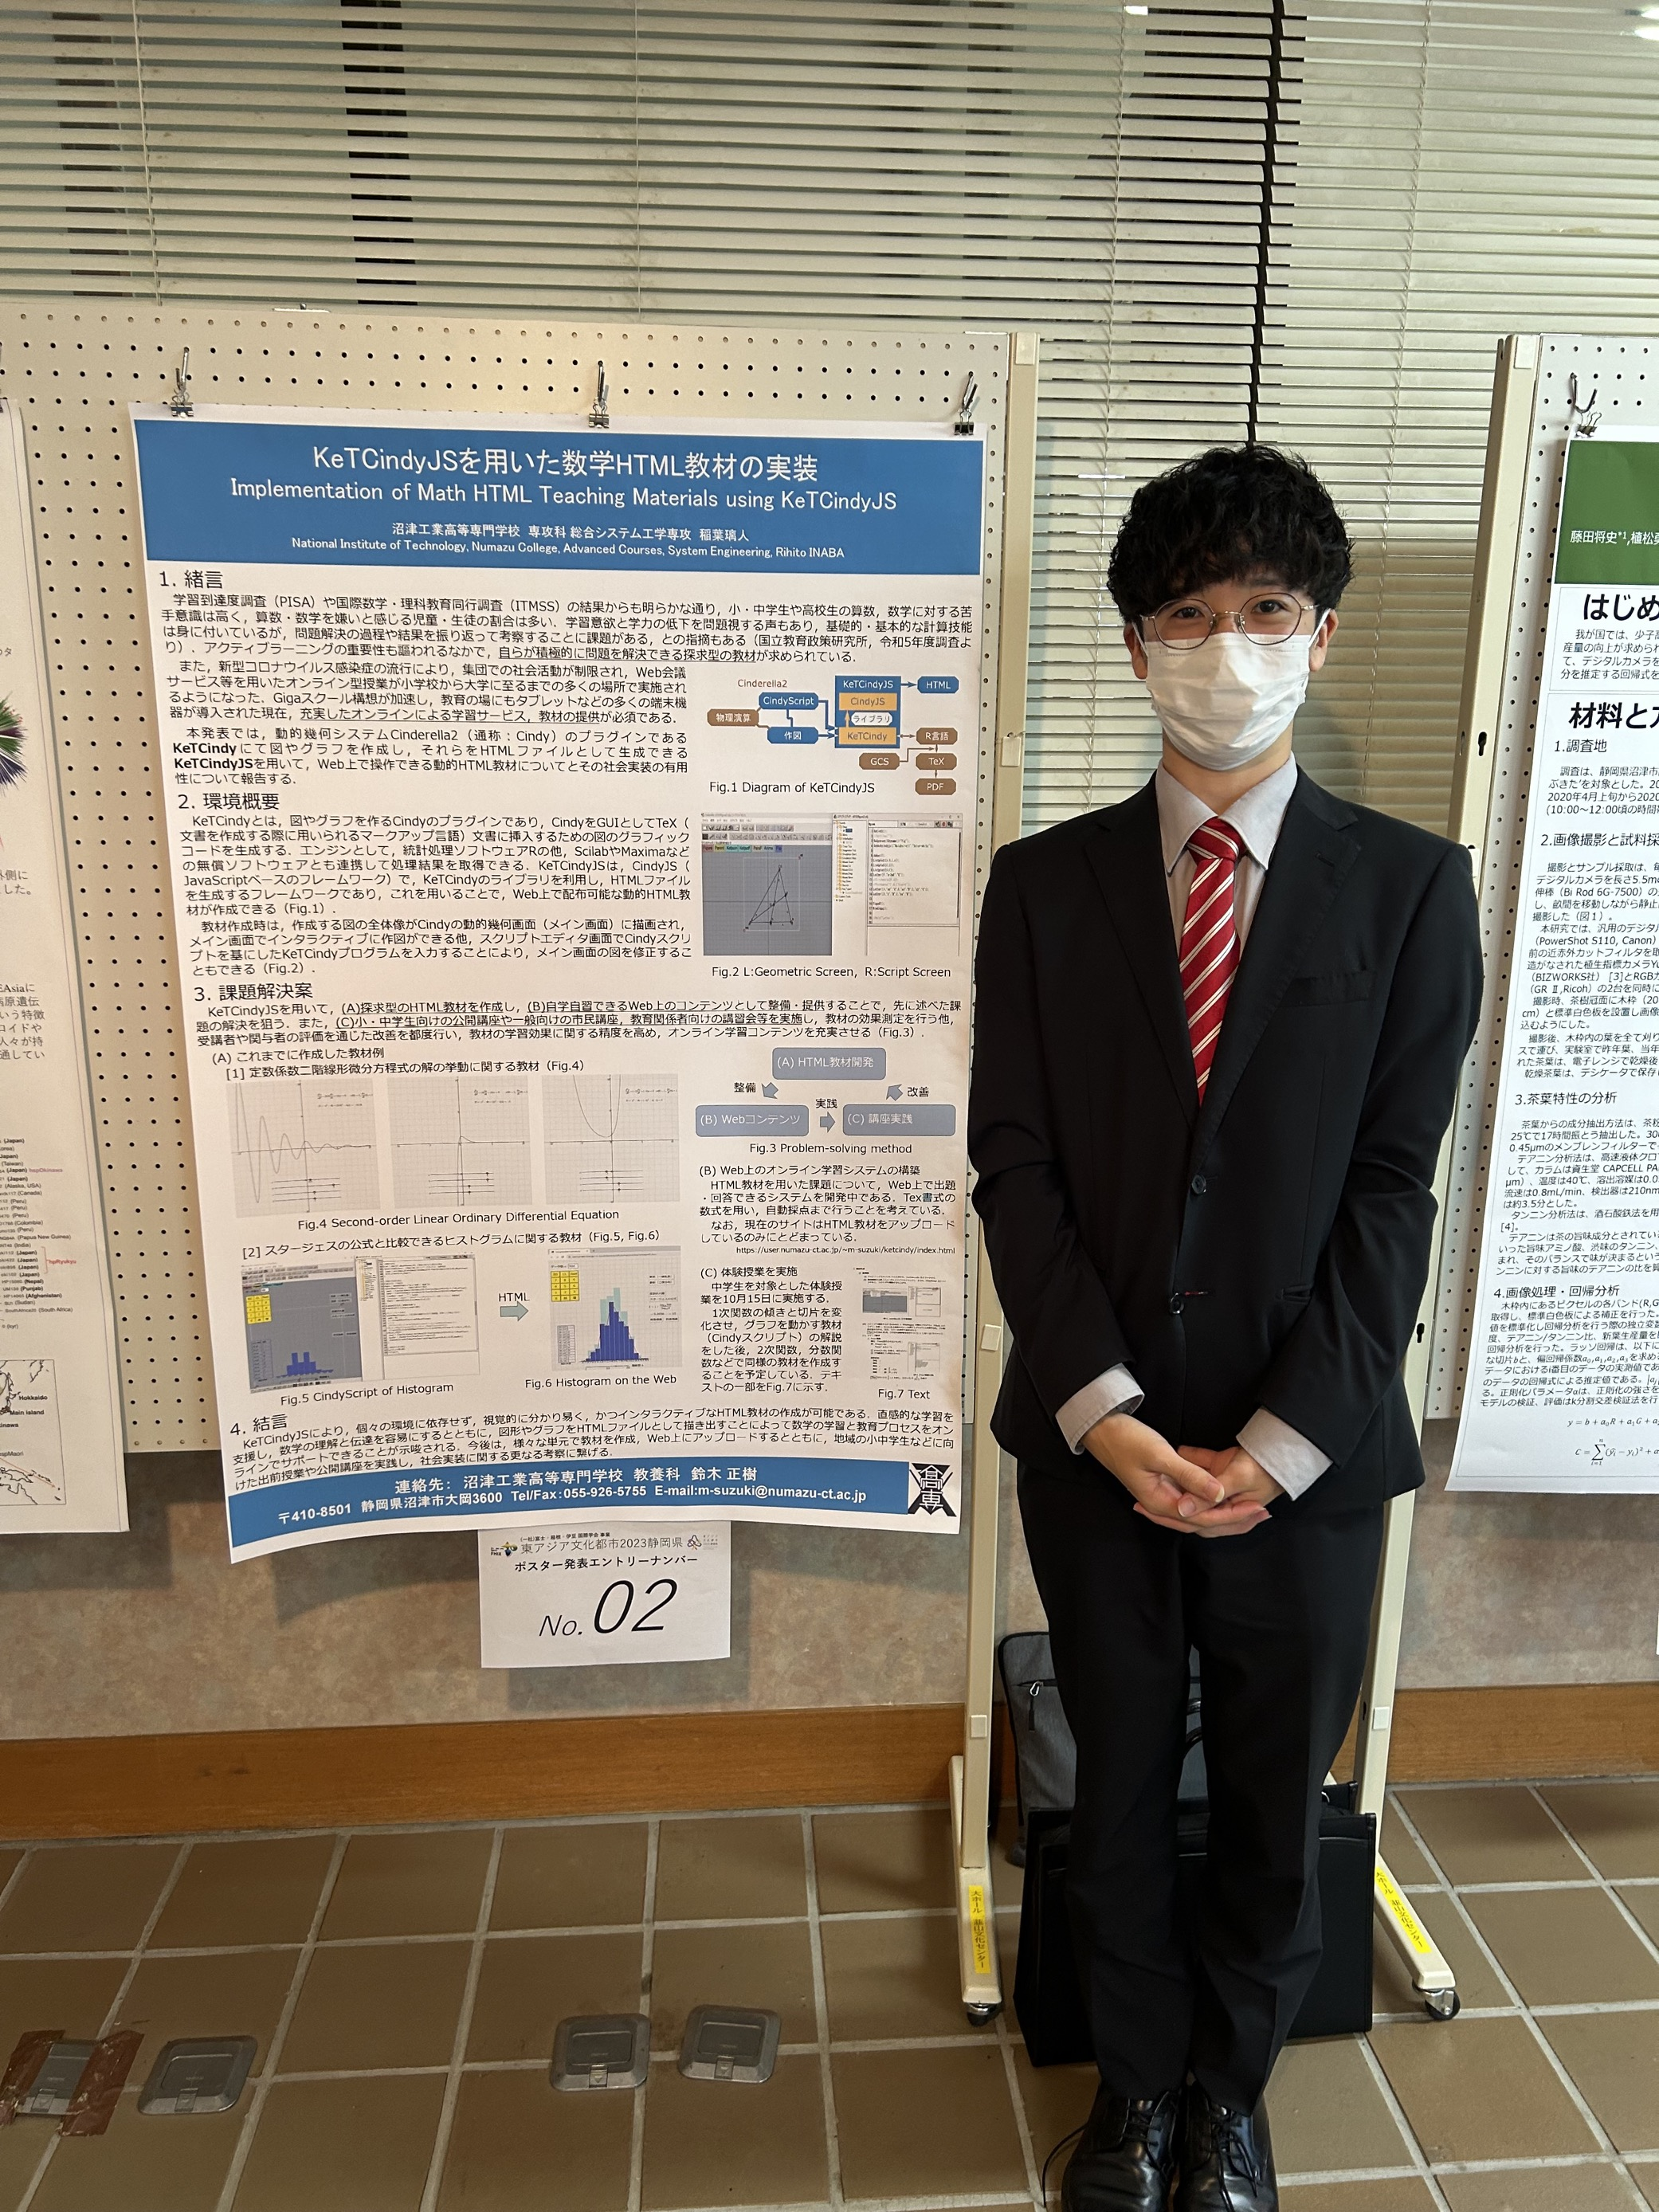
\includegraphics[scale=0.05]{img/ActiveReport/20231015_p.png}
    \end{column}
  \end{columns}
\end{frame}

\begin{frame}[t]{沼津高専ミニミニ体験授業 2024/6/9}
  沼津高専主催のイベント「ミニミニ体験」の1ブースにて,
  中学生50名を対象に,高専数学入試問題のワンポイントミニ授業が行われました.
  ミニ授業を通じて, これまでにKeTCindyJSを用いて開発した探求型数学HTML教材の
  有用性を確認することができました.
  \begin{columns}[T]
    \begin{column}{0.5\linewidth}
      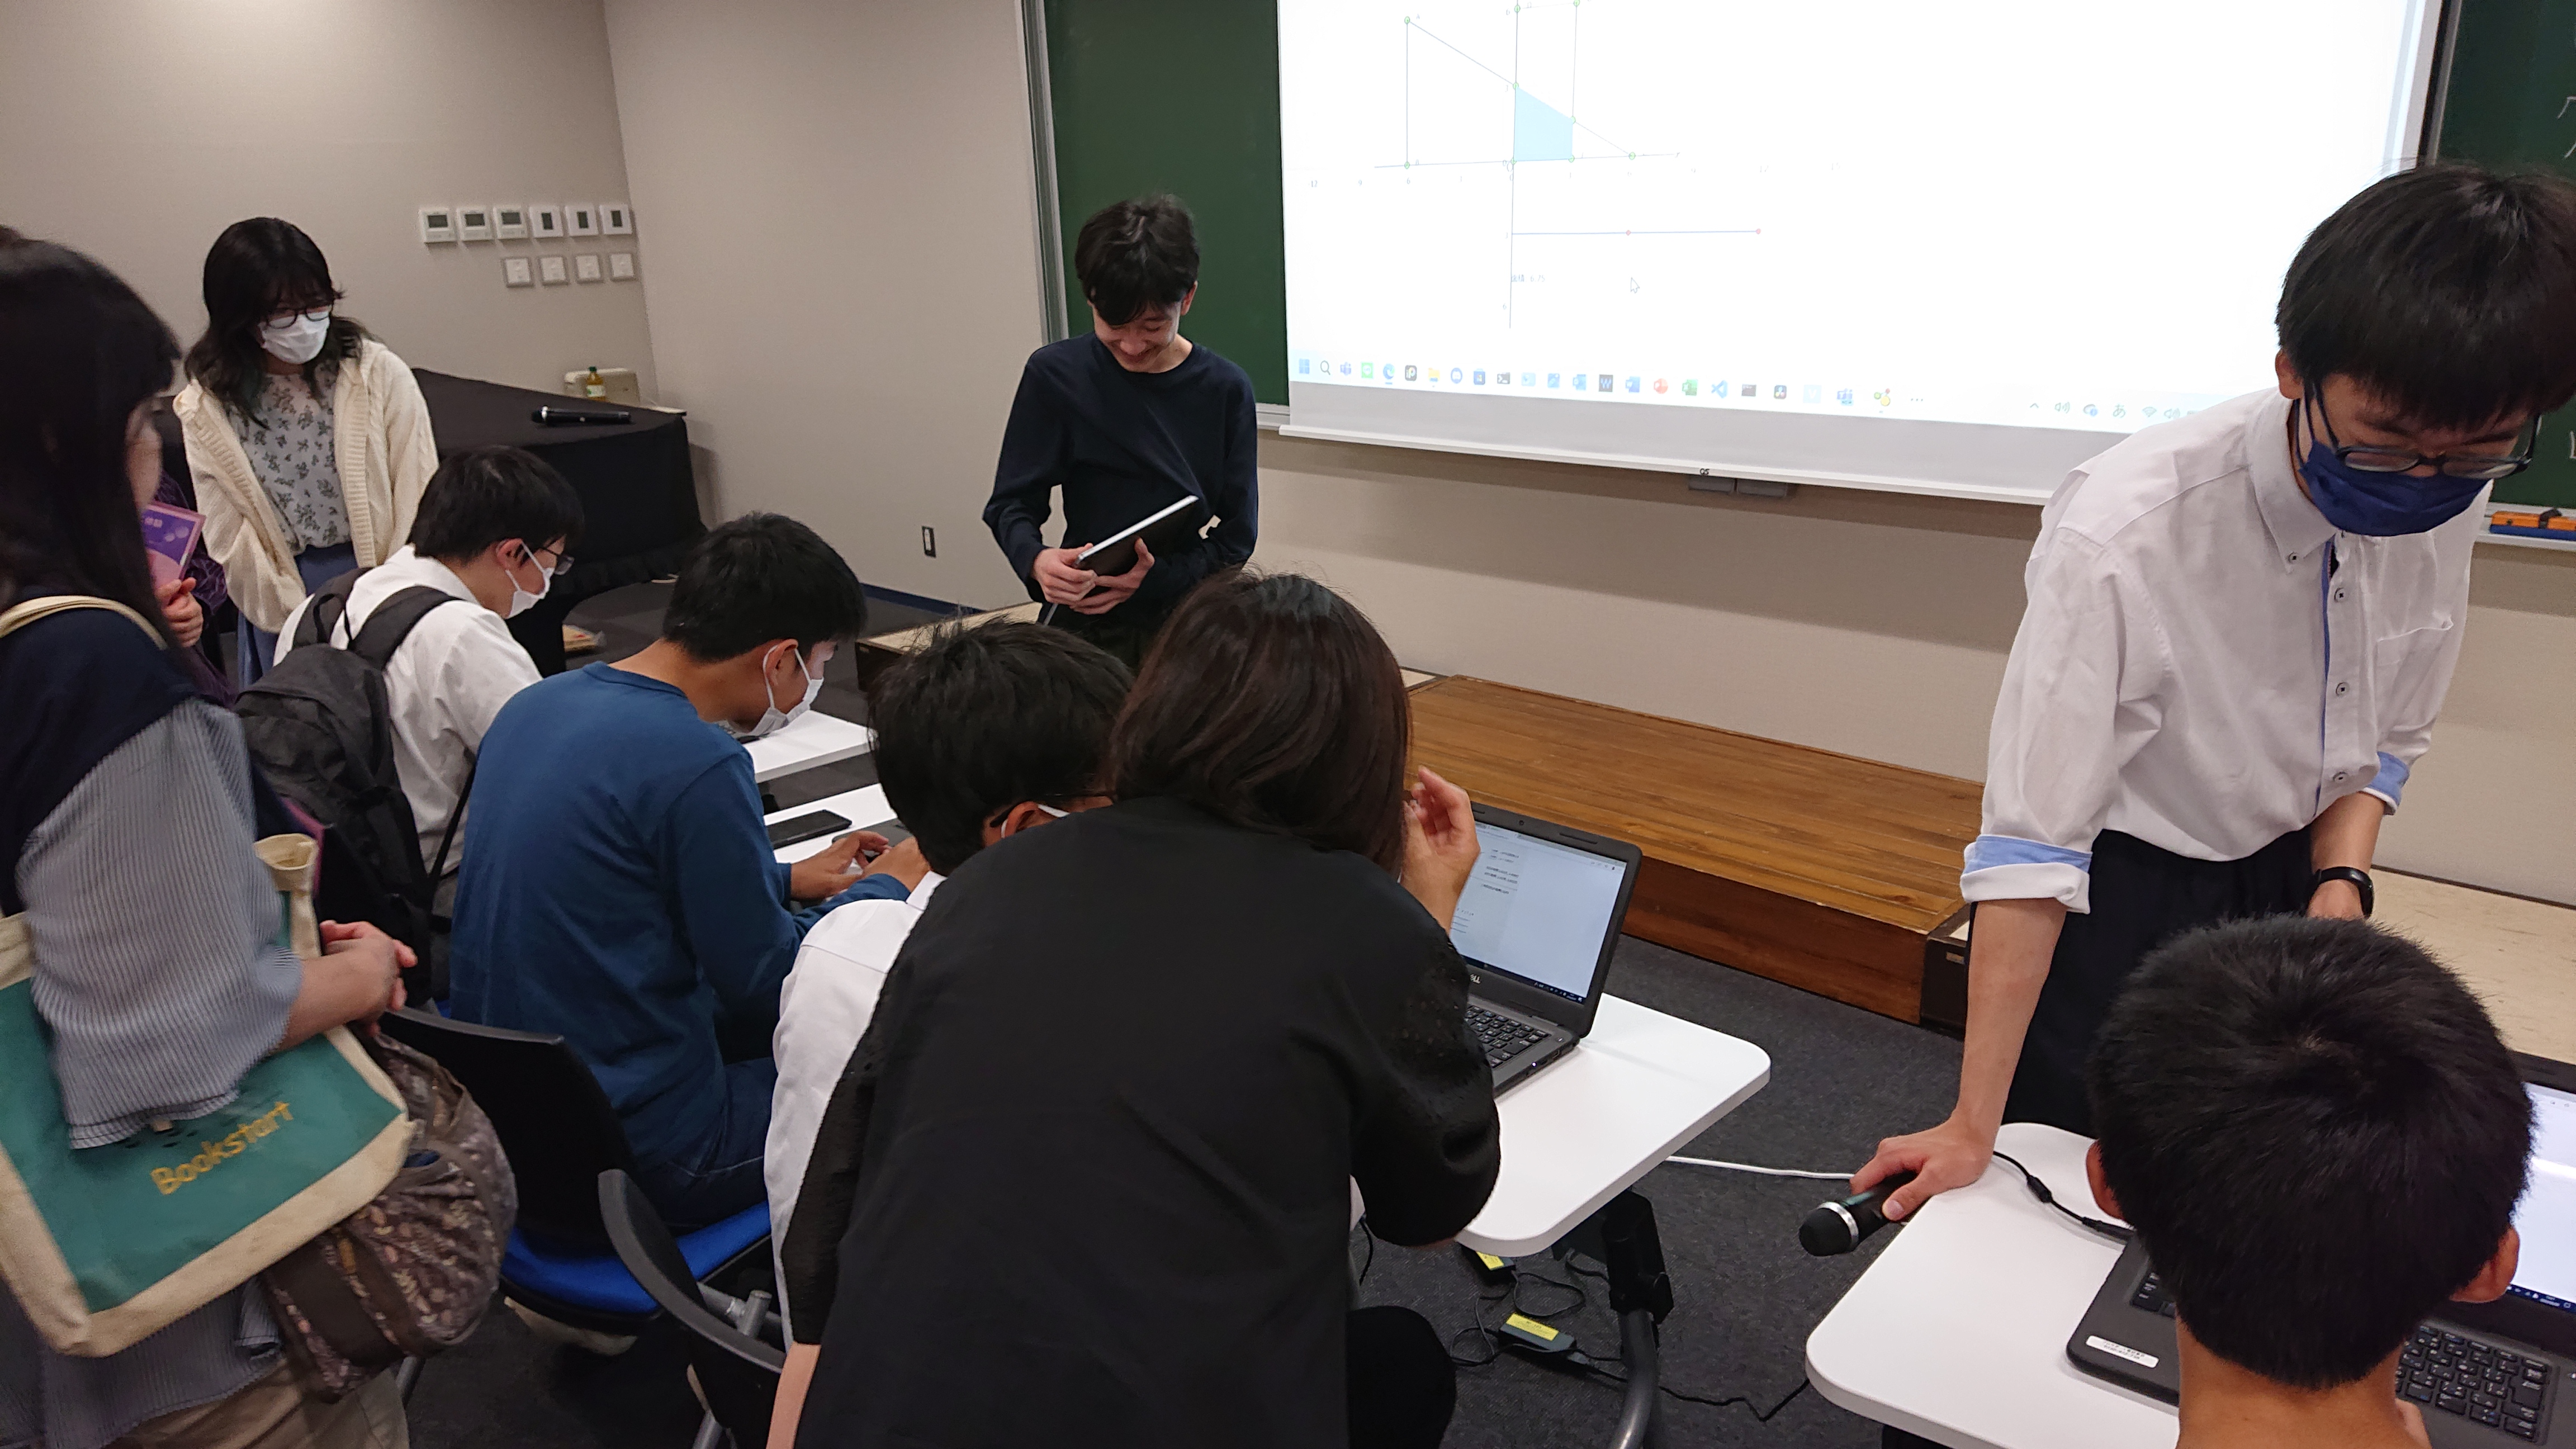
\includegraphics[width=\linewidth]{img/ActiveReport/20240609_minimini1.jpg}
    \end{column}
    \begin{column}{0.5\linewidth}
      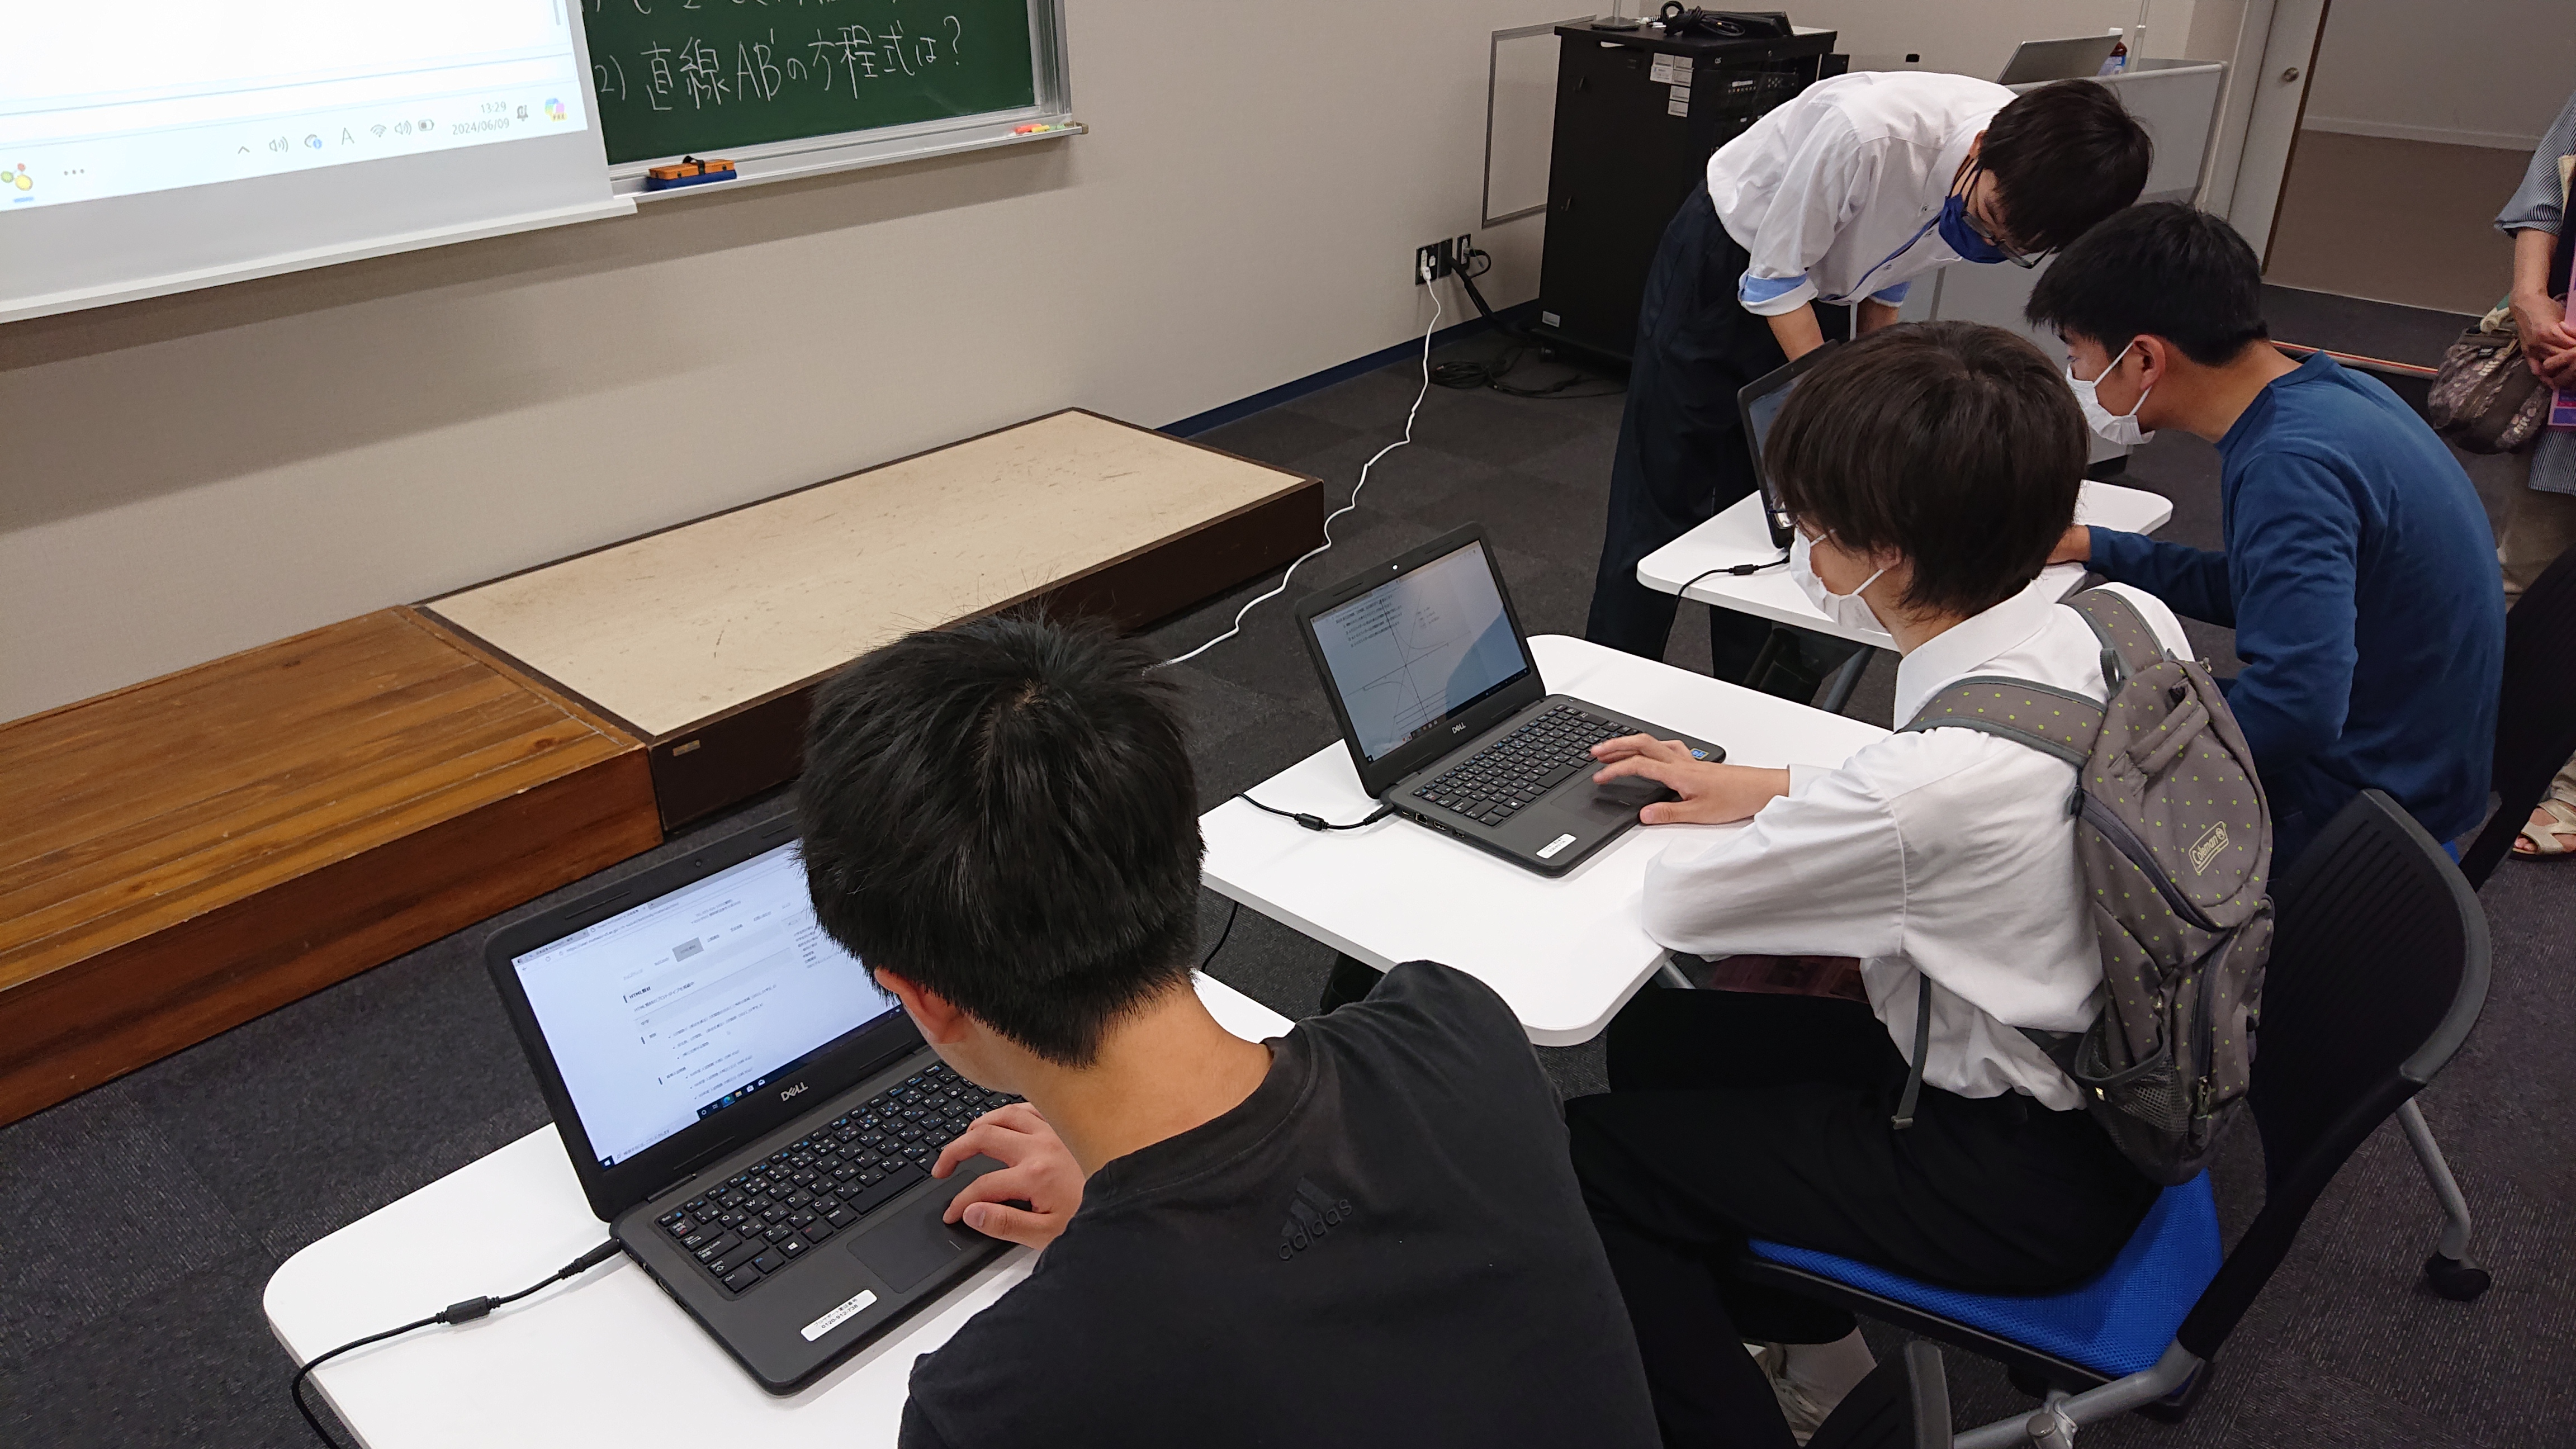
\includegraphics[width=\linewidth]{img/ActiveReport/20240609_minimini2.jpg}
    \end{column}
  \end{columns}
\end{frame}

\begin{frame}[t]{高専数学入試問題のワンポイントミニ授業 2024/08/03}
  沼津高専の一日体験入学にて, 「KeTCindy体験会」が開催されました.
  中学生30名, 高専生10名が参加し, Cindyスクリプトの解説を受けた後,
  各々の発想で関数のグラフや図形を作成しました.
  \begin{columns}[T]
    \begin{column}{0.5\linewidth}
      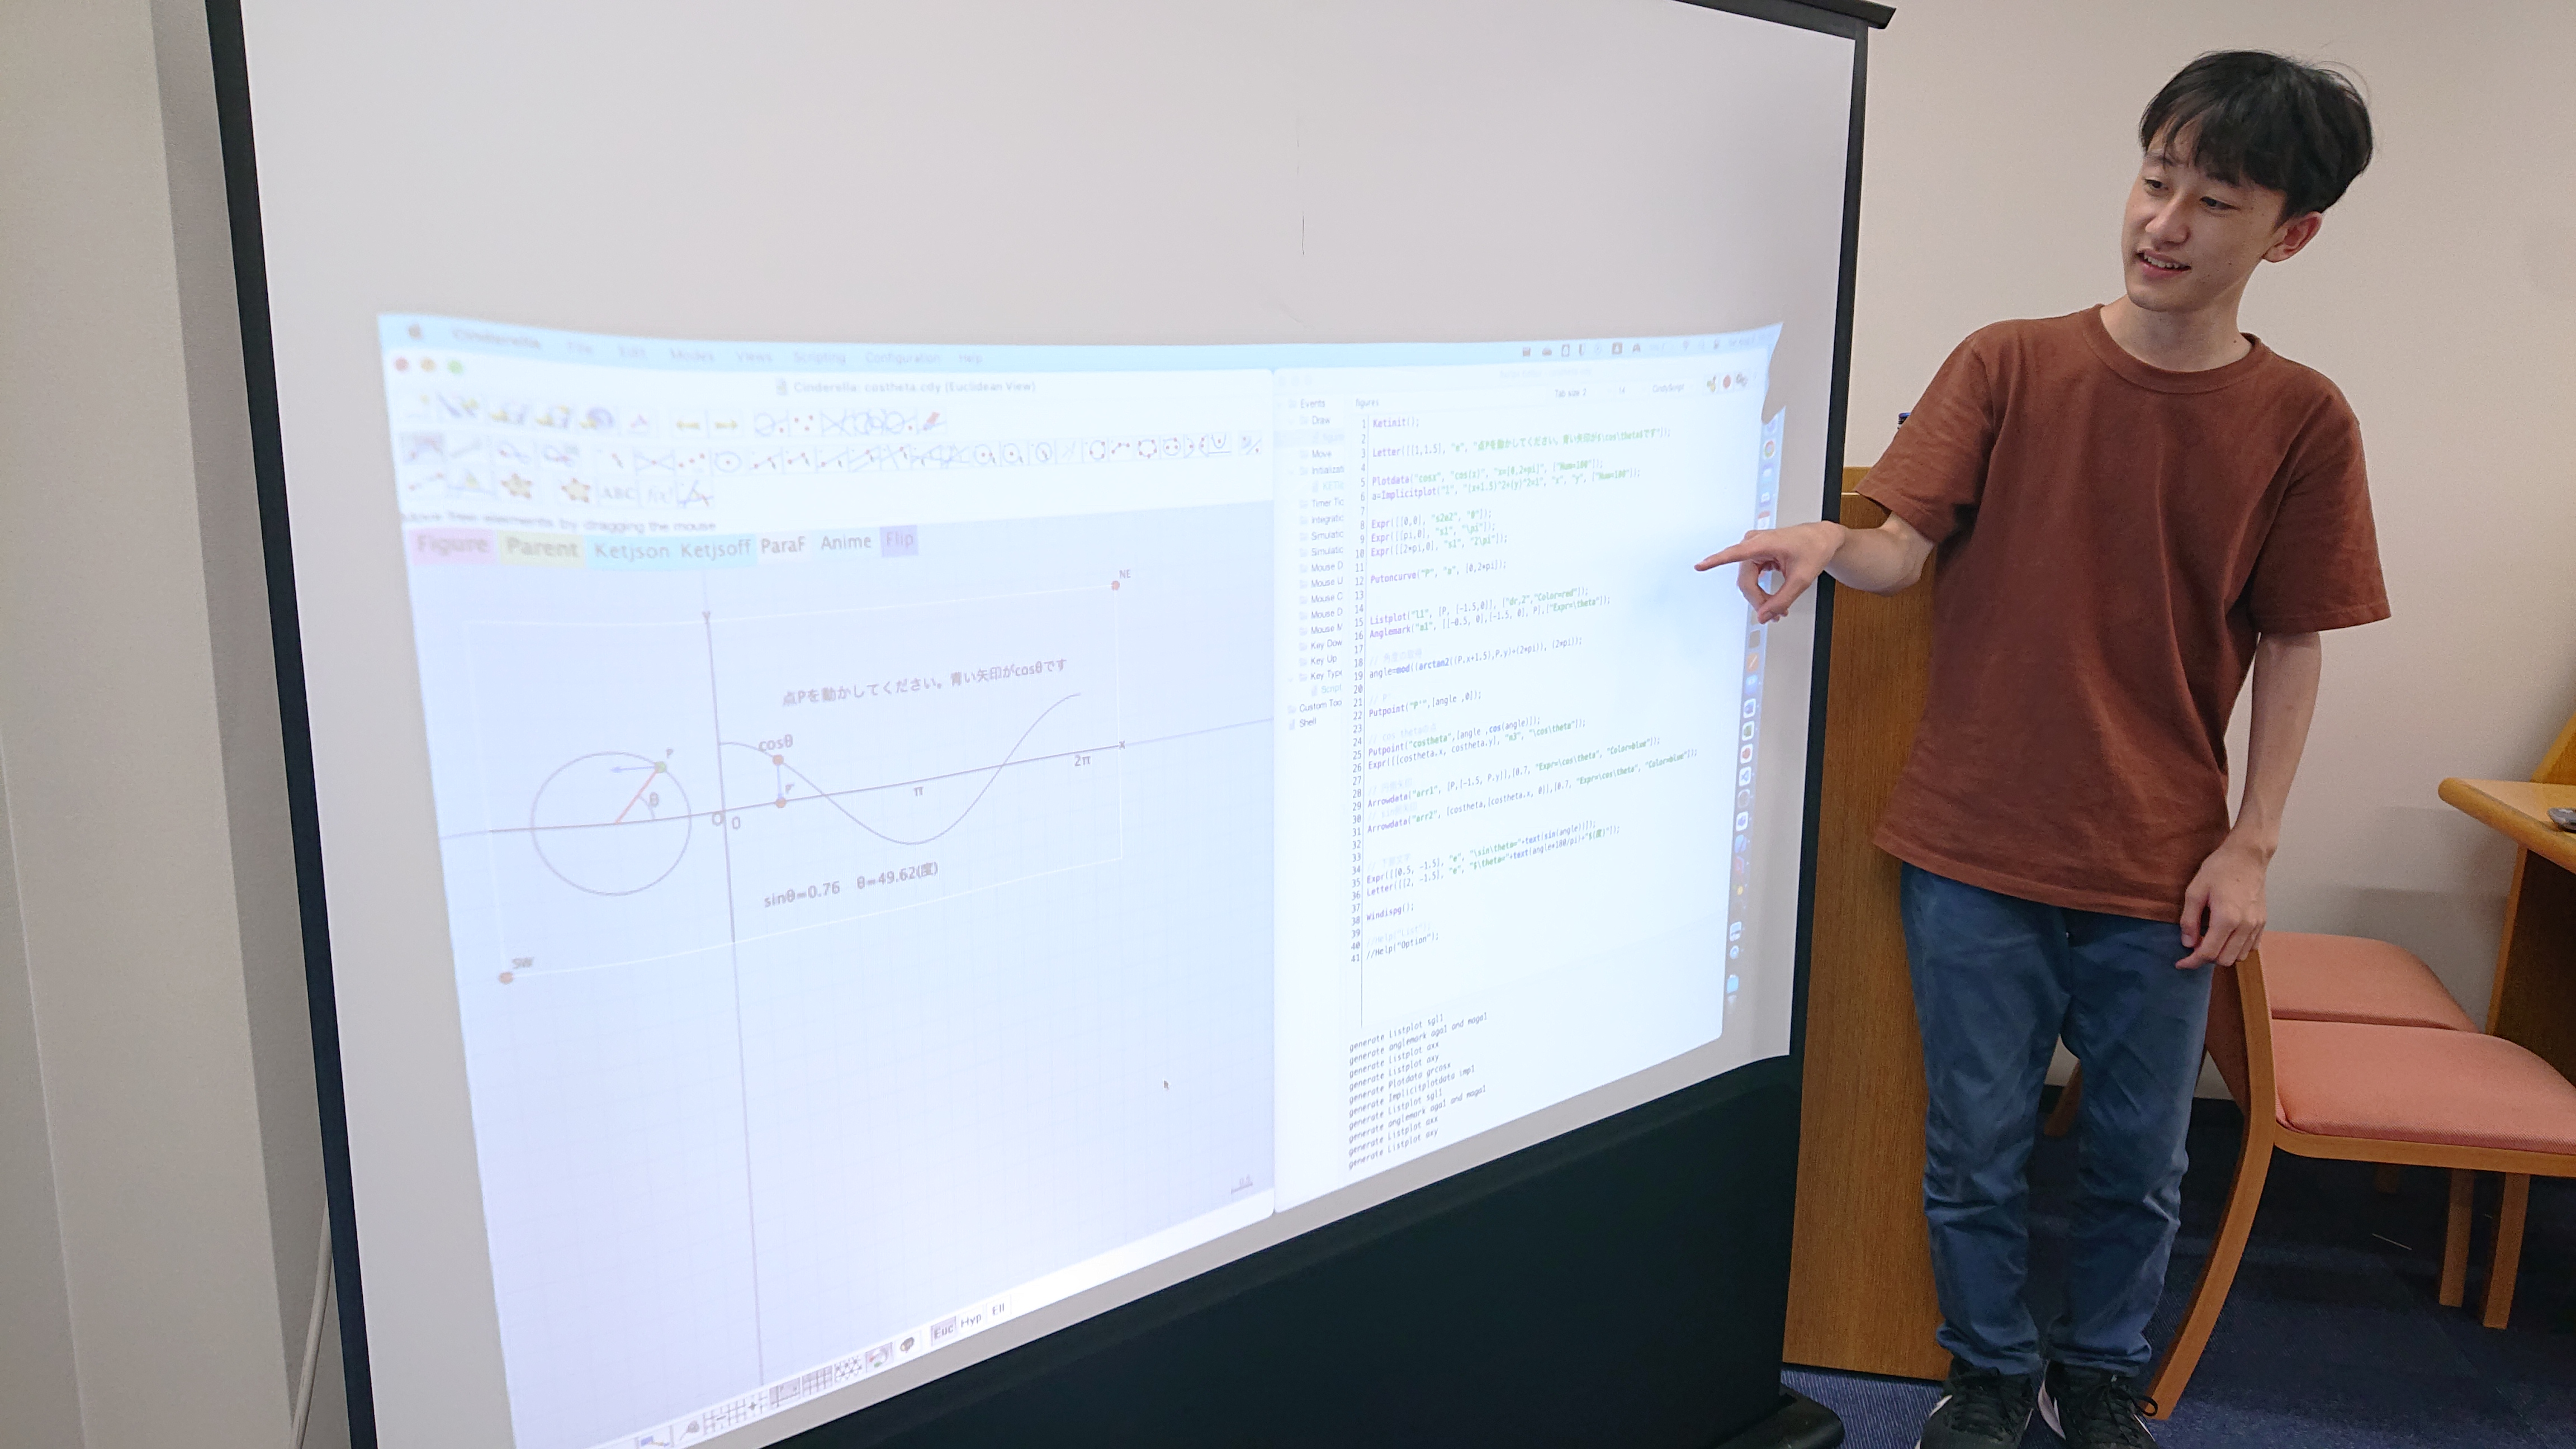
\includegraphics[width=\linewidth]{img/ActiveReport/20240803onepoint3.jpg}
    \end{column}
    \begin{column}{0.5\linewidth}
      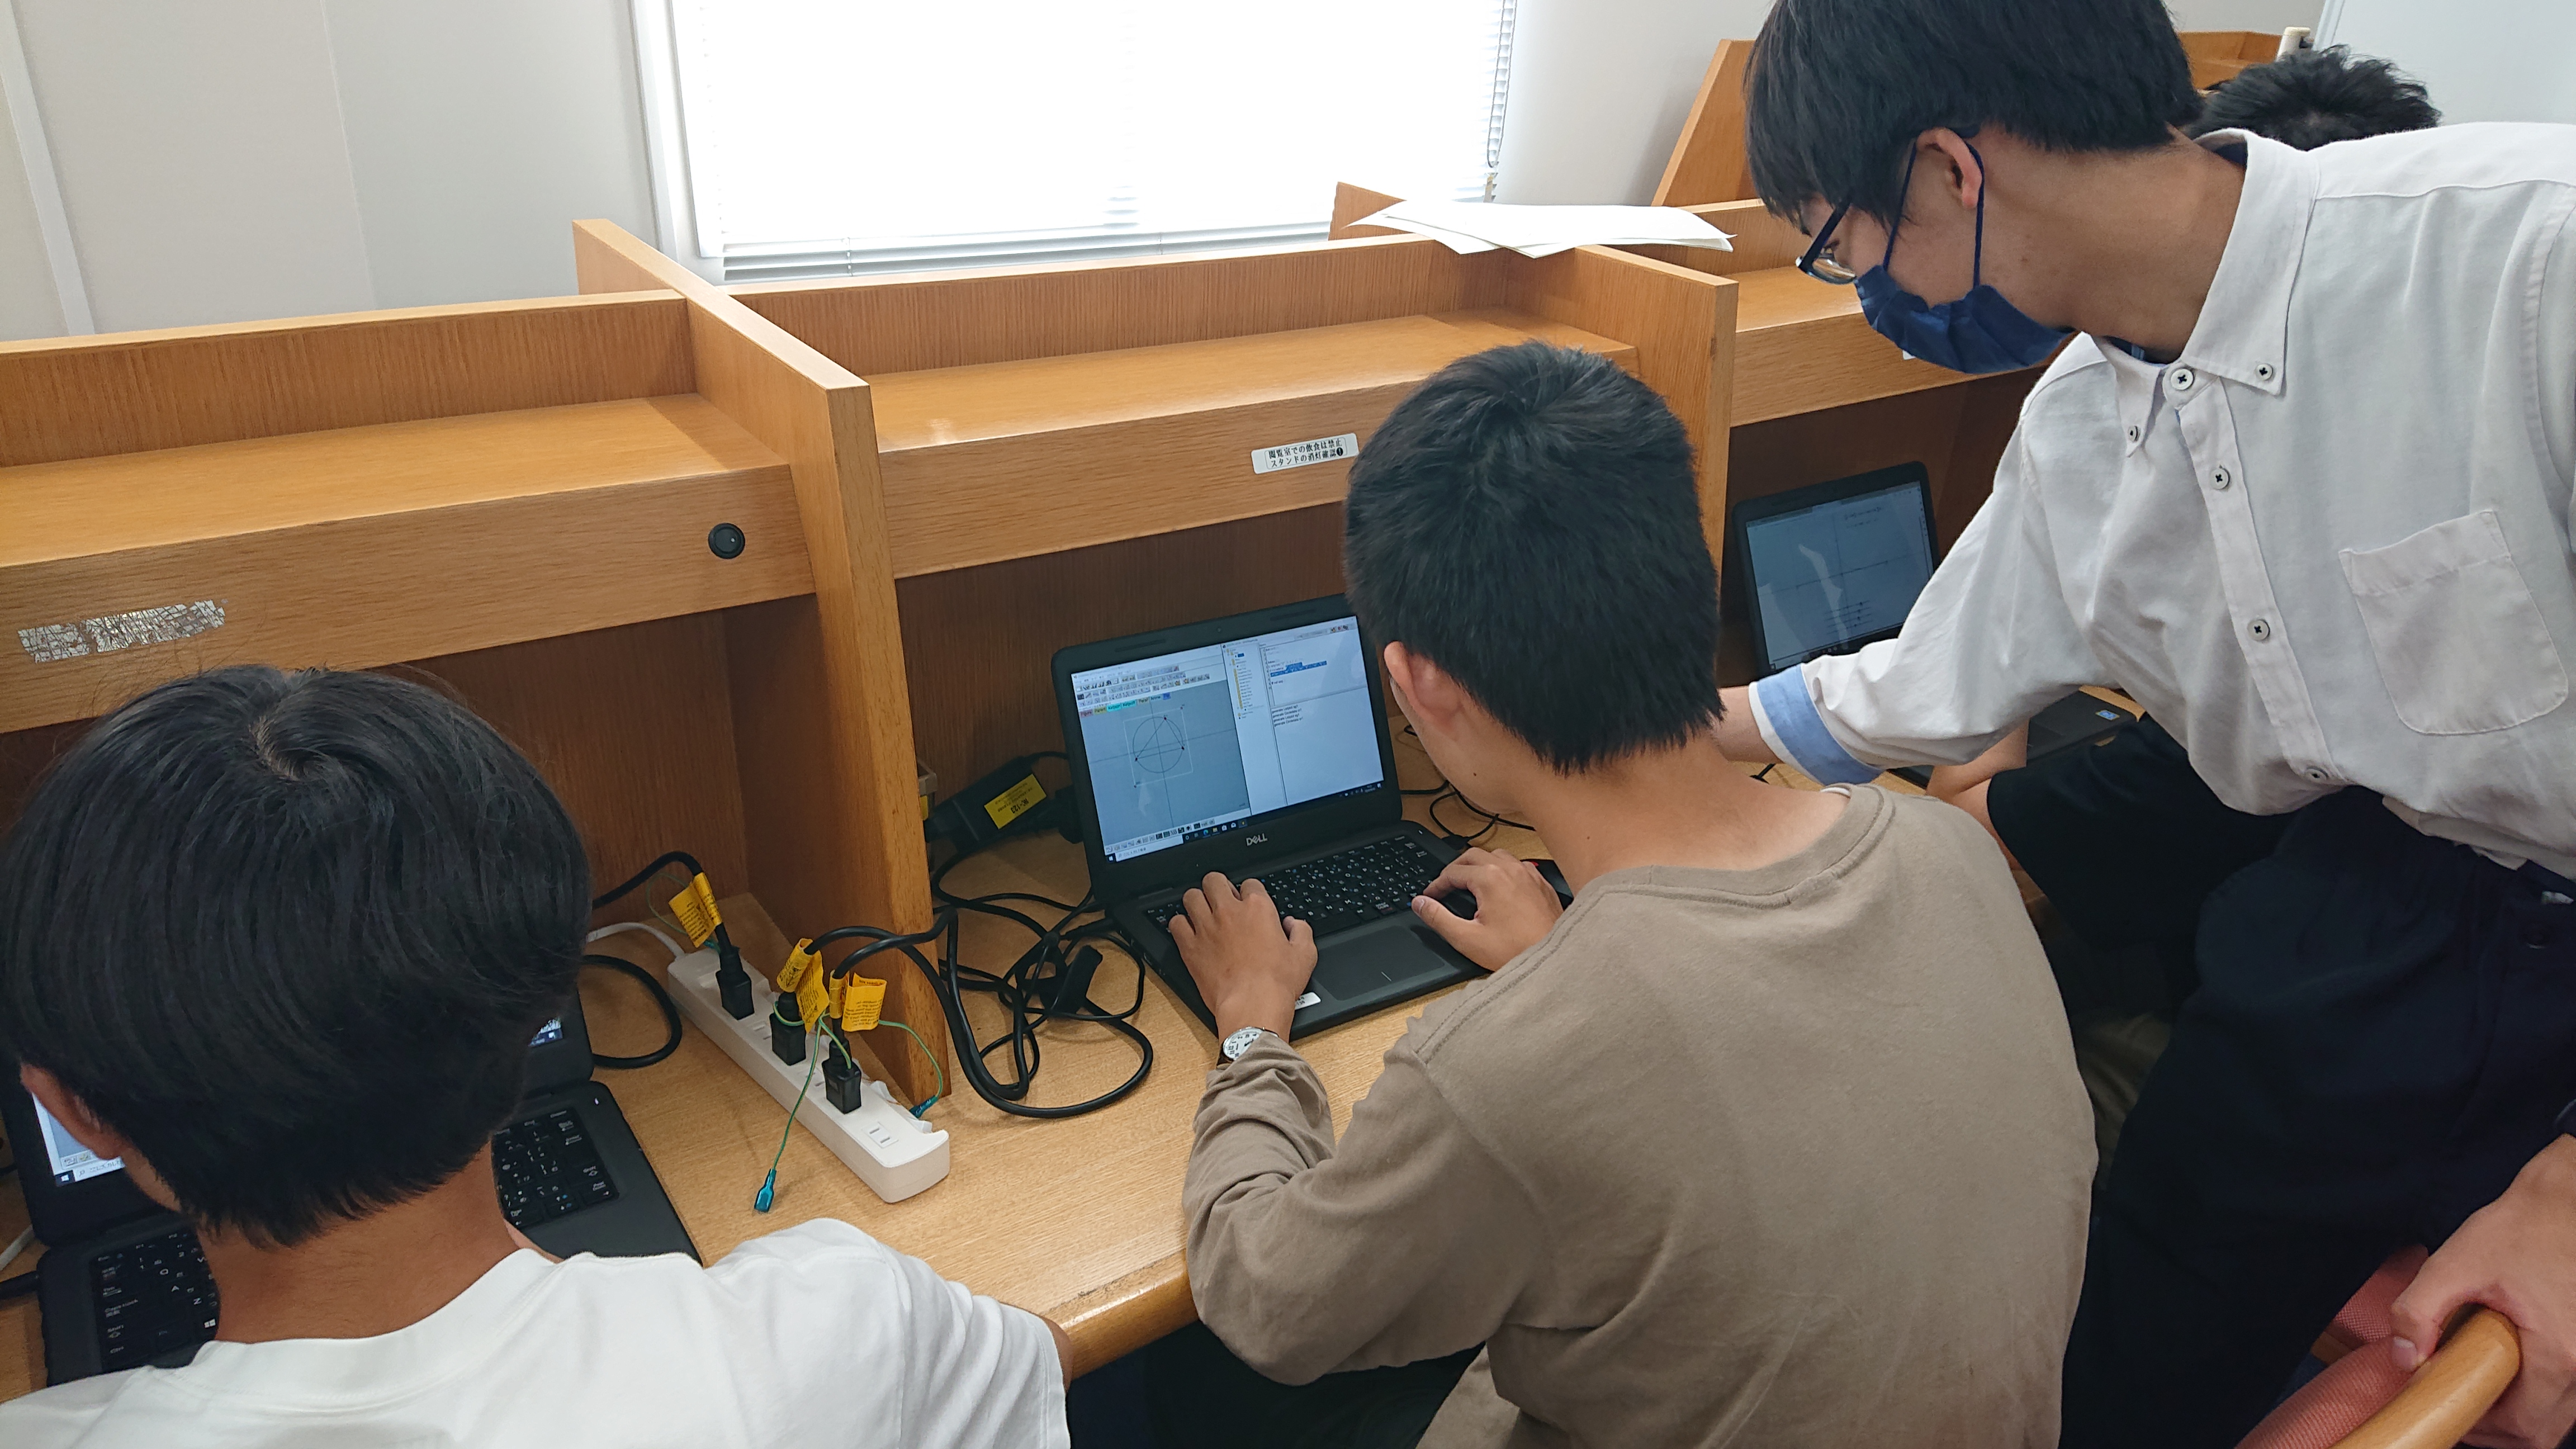
\includegraphics[width=\linewidth]{img/ActiveReport/20240803onepoint4.jpg}
    \end{column}
  \end{columns}
\end{frame}

\begin{frame}[t]{\bfseries Summary}
  \tableofcontents
\end{frame}

% \section{Summary}

\end{document}